\documentclass[12pt]{report}

%Packages
\usepackage[a4paper]{geometry}
\usepackage{graphicx}
\usepackage{algpseudocode}
\usepackage{algorithm}
\usepackage{hyperref}
\usepackage[xindy,acronym,nonumberlist=true]{glossaries}
\usepackage{xepersian}

\settextfont{XB Zar}

%Algorithm
\renewcommand{\algorithmicrequire}{\textbf{Input:}}
\renewcommand{\algorithmicensure}{\textbf{Output:}}

%Glossaries
\newglossarystyle{myFaToEn}{
	\renewenvironment{theglossary}{}{}
	\renewcommand*{\glsgroupskip}{\vskip 10mm}
	\renewcommand*{\glsgroupheading}[1]{\subsection*{\glsgetgrouptitle{##1}}}
	\renewcommand*{\glossentry}[2]{\noindent\glsentryname{##1}\dotfill\space \glsentrytext{##1}
		
	}
}
\newglossarystyle{myEntoFa}{
	\renewenvironment{theglossary}{}{}
	\renewcommand*{\glsgroupskip}{\vskip 10mm}
	\renewcommand*{\glsgroupheading}[1]{\begin{LTR} \subsection*{\glsgetgrouptitle{##1}} \end{LTR}}
	\renewcommand*{\glossentry}[2]{\noindent\glsentrytext{##1}\dotfill\space \glsentryname{##1}
		
	}
}
\newglossarystyle{myAbbrlist}{
	\renewenvironment{theglossary}{}{}
	\renewcommand*{\glsgroupskip}{\vskip 10mm}
	\renewcommand*{\glsgroupheading}[1]{\begin{LTR} \subsection*{\glsgetgrouptitle{##1}} \end{LTR}}
	\renewcommand*{\glossentry}[2]{\noindent\glsentrytext{##1}\dotfill\space \Glsentrylong{##1}
		
	}
	\renewcommand*{\acronymname}{\rl{فهرست اختصارات}}
}
\newglossary[glg]{english}{gls}{glo}{واژه‌نامه انگلیسی به فارسی}
\newglossary[blg]{persian}{bls}{blo}{واژه‌نامه فارسی به انگلیسی}
\makeglossaries
\glsdisablehyper
\let\oldgls\gls
\let\oldglspl\glspl
\makeatletter
\renewrobustcmd*{\gls}{\@ifstar\@msgls\@mgls}
\newcommand*{\@mgls}[1] {\ifthenelse{\equal{\glsentrytype{#1}}{english}}{\oldgls{#1}\glsuseri{f-#1}}{\lr{\oldgls{#1}}}}
\newcommand*{\@msgls}[1]{\ifthenelse{\equal{\glsentrytype{#1}}{english}}{\glstext{#1}\glsuseri{f-#1}}{\lr{\glsentryname{#1}}}}
\renewrobustcmd*{\glspl}{\@ifstar\@msglspl\@mglspl}
\newcommand*{\@mglspl}[1] {\ifthenelse{\equal{\glsentrytype{#1}}{english}}{\oldglspl{#1}\glsuseri{f-#1}}{\oldglspl{#1}}}
\newcommand*{\@msglspl}[1]{\ifthenelse{\equal{\glsentrytype{#1}}{english}}{\glsplural{#1}\glsuseri{f-#1}}{\glsentryplural{#1}}}
\makeatother
\newcommand{\newword}[4]{
	\newglossaryentry{#1}     {type={english},name={\lr{#2}},plural={#4},text={#3},description={}}
	\newglossaryentry{f-#1} {type={persian},name={#3},text={\lr{#2}},description={}}
}
\defglsentryfmt[english]{\glsgenentryfmt\ifglsused{\glslabel}{}{\LTRfootnote{\glsentryname{\glslabel}}}}
\defglsentryfmt[acronym]{\glsentryname{\glslabel}\ifglsused{\glslabel}{}{\LTRfootnote{\glsentrydesc{\glslabel}}}}
\newcommand{\printabbreviation}{
	\cleardoublepage
	\phantomsection
	\baselineskip=.75cm
	\addcontentsline{toc}{chapter}{فهرست اختصارات}
	\setglossarystyle{myAbbrlist}
	\begin{LTR}
		\Oldprintglossary[type=acronym]	
	\end{LTR}
	\clearpage
}
\newcommand{\printacronyms}{\printabbreviation}
\let\Oldprintglossary\printglossary
\renewcommand{\printglossary}{
	\let\appendix\relax
	\clearpage
	\phantomsection
	\twocolumn{}
	\addcontentsline{toc}{chapter}{واژه نامه انگلیسی به فارسی}
	\setglossarystyle{myEntoFa}
	\Oldprintglossary[type=english]
	\clearpage
	\phantomsection
	\addcontentsline{toc}{chapter}{واژه نامه فارسی به انگلیسی}
	\setglossarystyle{myFaToEn}
	\Oldprintglossary[type=persian]
	\onecolumn{}
}
\newword{pitch}{pitch}{نواک}{نواک‌ها}
\newword{velocity}{velocity}{شدت}{شدت‌ها}
\newword{timber}{timber}{دایره‌ی زنگی}{دایره‌های زنگی}
\newword{chord}{chord}{آکورد}{آکوردها}
\newword{sustain}{sustain}{نگه‌دارنده}{نگه‌دارنده‌ها}
\newword{sound wav}{sound wav}{موج صوت}{موج‌های صوت}
\newword{midi}{musical instrument digital interface}{رابط دیجیتال سازهای موسیقیایی}{رابطهای دیجیتال سازهای موسیقیایی}
\newword{pianoroll}{pianoroll}{رول پیانو}{رول‌های پیانو}
\newword{sheet music}{sheet music}{پارتیتور}{پارتیتورها}
\newword{duration}{duration}{کشش}{کشش‌ها}
\newacronym{MIDI}{MIDI}{Musical Instrument Digital Interface}

\begin{document}

\begin{figure}
    \centering
    
\includegraphics[height=2.5cm]{./statics/UT-Logo.pdf}
\end{figure}

\begin{center}
    پردیس علوم

    دانشکده ریاضی، آمار و علوم کامپیوتر
\end{center}

\vspace{1cm}

\begin{center}
    \huge{آوانویسی خودکار موسیقی بر مبنای یادگیری ژرف}
\end{center}

\vspace{1cm}

\begin{center}
    نگارنده
\end{center}
\begin{center}
    \textbf{آرمان مزدائی}
\end{center}

\begin{center}
    \begin{tabular}{rr}
        استاد راهنما:& دکتر باقر باباعلی
        \\
        استاد مشاور:& دکتر هومان اسعدی
    \end{tabular}
\end{center}

\vspace{3cm}
\begin{center}
    پایان نامه برای دریافت درجه کارشناسی ارشد

    در رشته علوم کامپیوتر
\end{center}

\begin{center}
تاریخ دفاع: شهریور ۱۳۹۹
\end{center}

\pagestyle{empty}
\pagenumbering{}

\newpage
\pagestyle{plain}
\setcounter{page}{1}
\pagenumbering{harfi}
\chapter*{چکیده}
هدف مسئله آوانویسی خودکار موسیقی، استخراج فرم نوشتاری موسیقی از روی موج صوت ضبط
شده از اجرای یک قطعه می‌باشد. به دلیل چالش‌هایی مانند گستردگی فضای خروجی، تفاوت
میان دایره‌زنگی سازهای مختلف و تداخل هارومونیک‌های صوتی این مسئله یکی از
سخت‌ترین مسائل حوزه بازیابی اطلاعات موسیقیایی می‌باشد.

با توجه به این که عمده داده موسیقیایی موجود به شکل موج صوت ذخیره شده است، داشتن
سیستمی که با قابلیت اطمینان بالا بتواند این اطلاعات را به فرم نوشتاری تبدیل کند
اهمیت بسیار بالایی دارد. همچنین حل بسیاری از مسائل حوزه بازیابی اطلاعات
موسیقیایی بر روی فرم نوشتاری موسیقی بسیار ساده‌تر است. درنتیجه دست‌یابی به یک
سیستم آوانویسی خودکار موسیقی که بتواند عملکرد خوبی داشته باشد، منجر به حل شدن
بسیاری از مسائله دیگر این حوزه می‌شود.

در بازشناسی خودکار گفتار استفاده از یک مدل زبانی در کنار مدل آوایی می‌تواند
عملکرد نهایی سیستم را به شدت افزایش دهد. موسیقی نیز مانند زبان طبیعی، ساختاری
کاملا قائده‌مند است و محققان بر این باور هستند که متخصصان موسیقی نه تنها با
استفاده از اطلاعات صوتی دریافتی بلکه بیشتر با بهره‌گیری از دانش موسیقیایی خود
فرآیند آوانویسی را انجام می‌دهد. با این وجود سیستم‌های موجود برای آوانویسی
خودکار موسیقی تنها بر اطلاعات موجود در سیگنال اکتفا می‌کنند و از مدلی جدا
برای تصحیح این تشخیص‌ها بر اساس ساختارهای موسیقیایی بهره نمی‌برند.

دلیل این عدم استفاده از یک مدل موسیقیایی را می‌تواند چالش‌های ذاتی این مسئله
دانست. به علت مشکلاتی همچنون طولانی بودن دنباله‌های ورودی و خروجی روش‌های موجود
برای استفاده از یک مدل موسیقیایی در کنار یک مدل آوایی عملا قابل استفاده
نمی‌باشند. در این پایان‌نامه تلاش شده است که یک روش نوین برای استفاده از مدل
موسیقیایی در کنار مدل آوایی، برای انجام آوانویسی خودکار موسیقی، بررسی شود و
عملکرد این روش با مدل آوایی تنها بررسی شود.
\tableofcontents

\newpage
\pagestyle{plain}
\setcounter{page}{1}
\pagenumbering{arabic}
\chapter{تعریف مسئله و مفاهیم مقدماتی}
\section{مروری بر موسیقی}
بدون شک موسیقی یکی از غنی‌ترین و قدیمی‌ترین بخش‌های تمدن بشری هست. اولین ساز
حدود چهل و پنج هزار سال پیش ساخته شد و تا امروز این شکل هنر به رشد خود ادامه‌
داده است. در این بخش مروری کوتاه بر مفاهیم موسیقیایی استفاده شده در این
پایان‌نامه انجام شده است.

\subsection{نت موسیقی}
مهم‌ترین بخش پایه‌ای موسیقی نت هست که می‌توان آن را با سه مفهوم \gls{pitch}،
\gls{velocity} و \gls{timber} توصیف کرد. \gls{pitch} فرکانس پایه‌‌ی صوت تولید
شده توسط ساز هست. \gls{pitch} واضح‌ترین فرکانس قابل درک نت هست. \gls{pitch}
زیرتر به معنی فرکانس بالاتر هست. \gls{velocity}، قدرت نواختن نت را مشخص می‌کند.
نت‌های که \gls{velocity} بالاتری دارند قابل درک‌تر هستند. همچنین معمولا نت اول
هر کلمه موسیقیایی \gls{velocity} بالاتری دارد. درنهایت \gls{timber} اشاره به شکل
سیگنال صوت تولید شده دارد. دو نت می‌توانند \gls{pitch} یکسانی داشته باشند ولی
شکلی که این نوسان انجام می‌شود متفاوت باشد. این تفاوت را با \gls{timber} ساز
بیان می‌کنند. \gls{timber} مفهومی هست که باعث تفاوت صدای سازهای مختلف می‌شود. در
شکل۱.۱ نمونه‌ای از \gls{timber} ساز ویولن نشان داده شده است.
\begin{figure}
    \centering
    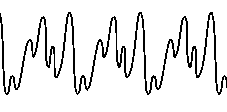
\includegraphics[height=2.5cm]{./statics/note_visualized.png}
    \caption{نمونه‌ای از \gls{timber} ویولن}
\end{figure}

همچنین هر نت یک زمان شروع یا onset و یک زمان پایان یا offset دارد. هرچند در بعضی
از سازها این مرزها کاملا مشخص و قابل تفکیک نمی‌باشند. برای مثال در پیانو پس از
رها کردن یک کلاویه همچنان ساز می‌تواند صوتی تولید کند.

وقتی از نواختن چند نت به صورت همزمان صحبت می‌کنیم معمولا مجموعه‌ای از نت‌ها با
هم صدایی خوش‌آیندتر تولید می‌کنند. به این مجموعه‌ی نت یک \gls{chord} گفته
می‌شود. یک \gls{chord} معمولا شامل نت‌هایی می‌شود که هارمونیک مشابه و نزدیک به
هم دارند. نت‌هایی که فرکانس پایه‌های آن‌ها با هم نسبت ۴، ۵، ۶ دارند نمونه‌ای از
یک \gls{chord} معروف هستند. به عنوان نمونه‌ای دیگر از \glspl{chord} مشهور
می‌توان به دو نت با نسب فرکانسی ۱ و ۲ اشاره کرد.

\subsection{پیانو}
پیانو یک ساز از خانواده ساز‌های صفحه‌کلیددار است که در سال ۱۶۹۸ اختراع شد. این
ساز در حالت استاندارد شامل ۸۸ کلید یا به اصلاح کلاویه هست که هرکدام نماینده یک
نت هستند. یکی از خصوصیات جالب این ساز این هست که پس از این که نوازنده شروع به
نواختن یک نت کرد تنها کنترلی که بر روی آن می‌تواند اعمال کنند یا رها کردن کلاویه
هست که باعث افت در شدت صدا می‌شود و یا دوباره نواخت همان نت هست.

همچنین این ساز شامل چندین پدال هست. مهمترین این پدال‌ها، پدال \gls{sustain} هست
که در صورتی که توسط نوازنده فشرده شده باشد، حتی رها کردن کلاویه باعث می‌شود صدای
آن نت باقی بماند. درنتیجه حتی اگه کلاویه متناظر یک نت هم فشرده نباشد باز آن نت
فعال می‌ماند.

\subsection{نمایش موسیقی}
همانند زبان طبیعی، برای موسیقی هم راه حلی نیاز هست که بتوان آن را ذخیره و به
سایرین منتقل کرد. همانند زبان طبیعی، نمایش‌های مختلفی نیز برای موسیقی وجود دارند
که بعضی‌ از آن‌ها مختص یک ساز خاص هستند. در ادامه سعی می‌شود چندتا از نمایش‌های
استفاده شده در این پایان‌نامه بررسی شوند.

\subsubsection{\gls{sound wav}}
از دید فیزیکی موسیقی چیزی بجز تغییر در فشار هوا و نوسان ذرات ماده نیست. با کمک
پیشرفت تکنولوژی می‌تواند از نوسانات را طی اجرای یک قطعه موسیقی در طول زمان
اندازه گرفت و با ایجاد مجدد نوسانات مشابه موسیقی را باز تولید کرد.

از این نمایش بیشتر در بحث‌های پردازش سیگنال مورد توجه قرار می‌گرد. برای استفاده
از این نمایش در کامپیوتر ابتدا نیاز هست تا این نمایش گسسته‌سازی شود.

\subsubsection{\gls{midi}}
در یک فایل \gls{MIDI} شروع، پایان، شدت، نواک و بسیاری دیگر از اطلاعات مربوط به
یک نت را می‌توان ذخیره کرد. همچنین این نمایش راه‌کارهایی برای تغییرات پدال‌ها و
سایر اطاعات اضافه نیز دارا می‌باشد. در نتیجه یک فایل \gls{MIDI} تمام اطاعات لازم
برای باز اجرای کامل یک قطعه موسیقی را دارا می‌باشد. با این حال این نمایش خوانایی
کمی‌ دارد و ساختار کلی موسیقی را رعایت نمی‌کند. برای همین استفاده از این نمایش
محدود به ارتباط بین ابزارهای دیجیتال هست.

\subsubsection{\gls{pianoroll}}
\gls{pianoroll} نمایشی دیگری هست که به صورت سنتی برای اجرای موسیقی به صورت
خودکار استفاده می‌شده است. این نمایش یک رول بزرگ هست که هر سطح این رول نماینده
یک زمان و هر ستون آن نماینده یک نت هست. خانه‌هایی که نت در آن‌ها فعال بود سوراخ
می‌شد تا ماشین بتواند آن را اجرا کند. با پیشرفت تکنولوژی این نمایش هم پیشرفت کرد
و بسیاری از نرم‌افزارهای مدرن از آن برای نمایش موسیقی استفاده می‌کنند.

به صورت کلاسیک این نمایش راهی برای نگه‌داری \gls{velocity} هر نت ندارند. برای
همین امروزه این اطلاعات به صورت جداگانه نگه‌داری می‌شوند. همچنین اطلاعاتی مثل
پلادها نیز در این نمایش جایی ندارند.
\begin{figure}
    \centering
    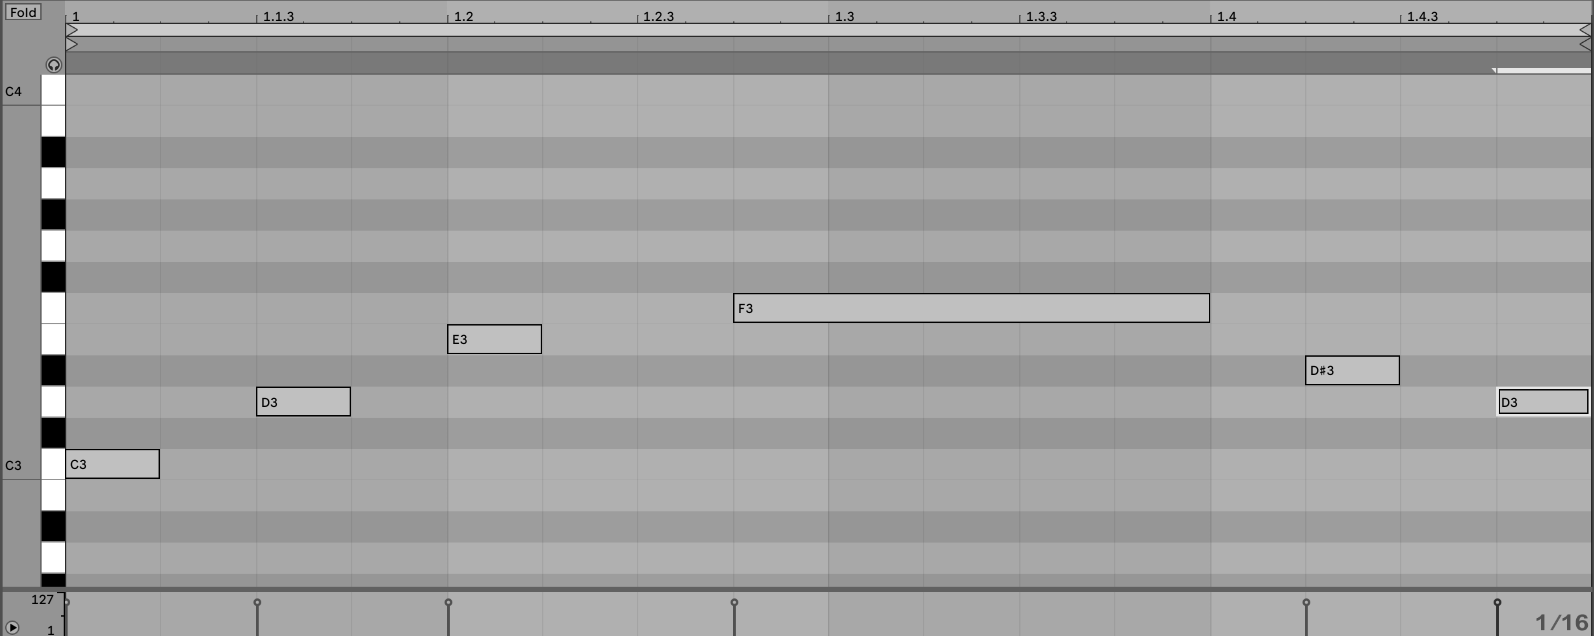
\includegraphics[width=12cm]{./statics/midi_piano_roll.png}
    \caption{نمونه‌ای از یک \gls{pianoroll} در یک نرم‌افزار کامپیوتری}
\end{figure}

\subsubsection{\gls{sheet music}}
این نمایش نمایشی هست که در مدارس موسیقی آموزش داده می‌شود و عمدتا به عنوان شکل
نوشتار استاندارد موسیقی شناخته می‌شود. بررسی کامل این نمایش خارج از دامنه‌ این
پایان‌نامه هست و به صورت مستقیم در این پایان‌نامه استفاده نمی‌شود. به صورت خلاصه
در این شکل از نمایش مجموعه \glspl{pitch}‌ مجاز و \glspl{duration}‌ مجاز مشخص
می‌شوند. سپس هر نت با توجه به مقدارهای تعریف شده بر روی خط‌های حامل نمایش داده
می‌شود.
\begin{figure}
    \centering
    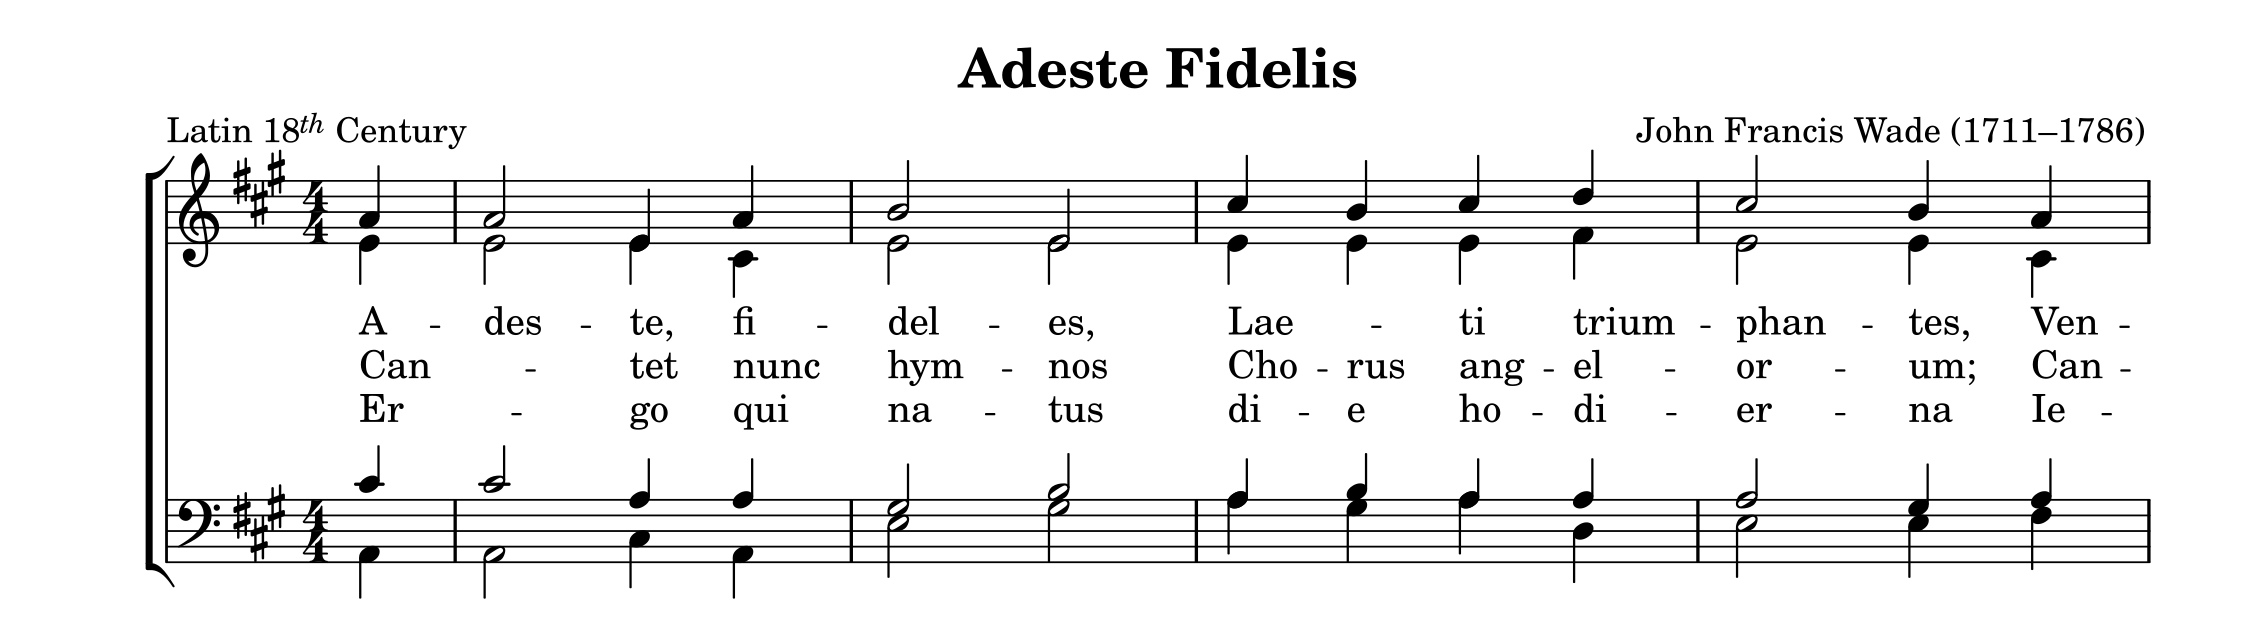
\includegraphics[width=12cm]{./statics/sheet_music.png}
    \caption{نمونه‌ای از یک \gls{sheet music}}
\end{figure}

\section{بازیابی اطلاعات موسیقیایی}
پیشرفت‌های تکنولوژی مانند شبکه، دیسک فشرده، ذخیره‌سازی ابری و موارد مشابه باعث
ایجاد حجم عظیمی داده در شکل‌های مختلف شده است. با توجه به این حجم از داده، نیاز
به سیستم‌هایی خودکار جهت استخراج اطلاعات از این داده‌ها کاملا مشهود است. یک
خانواده روش‌های موجود برای طراحی این سیستم‌ها، روش‌های \gls{cbir} هستند. این
روش‌ها به ما امکان می‌دهند که بر روی داده‌های چندرسانه‌ای به جست‌وجو بپردازیم که
از ضعف‌های سیستم‌های جست‌وجوی فعلی است. در چند دهه اخیر \gls{CBIR} یکی از
موضوعات پرطرفدار جهت مطالعه بوده است و ابزارهای مختلف زیادی نیز در این حوزه
توسعه یافته است که برای مثال می‌توان به \gls{qbic} اشاره کرد. همچنین تکنولوژی
\gls{mir} کمک کرده است تا اطلاعات مورد نیاز از روی سیگنال‌های صوتی به دست آید.
به صورت کلی یک سیگنال صوتی، پدیده‌ای بسیار پیچیده است، زیرا شامل حجم زیادی
اطلاعات مرتبط با هنرمند، ژانر، احساس، ساز و غیره است. با توجه به تنوع بالا
اطلاعات موجود در این سیگنال‌ها، حیطه‌ی گسترده‌ای از مطالب در \gls{cbmir} جهت
مطالعه و بررسی موجود می‌باشد.

برای \gls{cbmir} کاربردهای زیادی مانند مجموعه موسیقی شخصی‌سازی شده، توصیه
موسیقی، دسته‌بندی موسیقی، محافظت حق چاپ و غیره می‌توان متصور شد. برای توسعه این
کاربردها نیاز است که \gls{metadata} مورد نیاز از فایل‌های موسیقی استخراج شود ولی
از آن جا که متاسفانه این اطلاعات بر روی حجم زیادی از فایل‌های موسیقی قرار داده
نشده‌اند تنها راه موجود استخراج آن‌ها از روی سیگنال‌های صوتی است. همچنین انتظار
می‌رود \gls{CBMIR} برای مسائل زیر راهکاری داشته باشد:
\begin{itemize}
    \item تشخیص نواحی وکال در یک قطعه
    \item تشخیص هنرمند، سبک و نوع یک قطعه
    \item دسته بندی قطعات به دسته‌هایی مانند راک، جز، فولک، کلاسیک و غیره
    \item نوشتن خودکار متن یک آهنگ
    \item دسته بندی بخش‌های یک قطعه بر اساس بار احساسی آن بخش
    \item تشخیص نوع سازهای استفاده‌شده در یک قطعه مانند زهی، کوبه‌ای و غیره
    \item پیدا کردن قطعه‌های مرتبط به یک جستار به کمک معیارهای شباهت	
\end{itemize}

در ادامه به صورت خلاصه به معرفی بعضی از مهمترین مسائل این حوزه می‌پردازیم:

\subsection{قسمت‌بندی آواز و غیر آواز}
یک سیگنال صوتی از بخش‌های آواز، سازی، سکوت و یا ترکیب آواز و سازی تشکیل شده است.
تشخیص ساختاری یکی از مسائل جالب در این حوزه است. تشخیص نواحی سکوت یکی از اولین
قدم‌ها در هر سیستم پردازش گفتار و تشخیص صوت است. به صورت کلی طول بخش سکوت در هر
قطعه قابل چشم پوشی است زیرا بیش از ۹۹ درصد یک قطعه با صدای خواننده یا صدای ساز
پر شده است. بخش مشکل مسئله تشخیص آواز از صدای ساز است که در یک سیگنال موسیقی در
هم تنیده شده‌اند و بخش آوازی معمولا با یک موسیقی پس زمینه همراهی می‌شود. این
قسمت بندی پیش نیاز حل مسائل دیگری مانند تشخیص خواننده، تشخیص بار احساسی، تشخیص
ساز و رونویسی متن آواز است.

\subsection{تشخیص هنرمند}
هنرمند یکی از مهم‌ترین اجزای هر قطعه موسیقایی است. تشخیص خواننده، آهنگساز و
نوازنده از شاخه‌های این مسئله هست. در اکثر مواقع، سبک یکتای هر هنرمند، توسط
متخصصان قابل تمیز است. اگر با صدای یک خواننده آشنا باشید تنها با گوش دادن به بخش
کوتاهی از یک قطعه توانایی تشخیص خواننده را دارید. در حال حاضر فروشگاه‌های موسیقی
نیاز به کمک‌گیری از متخصصان دارند تا این اطلاعات را برای آن‌ها مشخص کنند ولی این
برای میلیون‌ها قطعه کاری طاقت فرسا و گاها غیرقابل اعتماد است. از کاربردهای چنین
سیستمی می‌توان به توصیه آهنگ‌های جدید، دسته‌بندی قطعات و حفاظت از حقوق ناشر
اشاره کرد.

\subsection{دسته‌بندی ژانر}
ژانر یکی دیگر از مفاهیم مهم برای دسته‌بندی قطعات موسیقی است و حجم عظیمی از
فروشگاه‌های موسیقی قطعات خود را بر اساس ژانر دسته‌بندی می‌کنند. این دسته‌بندی
معمولا بر اساس الگوهای موسیقیایی و سازهای استفاده شده انجام می‌شود. در حالی که
این تقسیم‌بندی برای شنوندگان عادی مسئولیت ساده‌ای نیست متخصصان بر اساس تجربه و
مهارت این مهم را انجام می‌دهند.

\subsection{جست‌وجو با زمزمه}
عکس و صوت پراستفاده‌ترین نوع محتوای چندرسانه‌ای هستند. در حاضر موتورهای جست‌وجوی
متنی به صورت گسترده استفاده می‌شوند و به صورت مستقیم در دسترس کاربران هستند. با
این حال زمانی که جست‌وجو بر روی داده‌های چندرسانه‌ای باشد، تبدیل جستار
چندرسانه‌ای به جستاری متنی فرآیندی پیچیده است و همچنین برای مواردی مانند پیدا
کردن یک قطعه موسیقی از طریق زمزمه موزیک آن شدنی نیست. به کمک یک سیستم
\gls{CBMIR} می‌توان جست‌وجوهایی از این دست را ممکن کرد.

\subsection{تشخیص بار احساسی}
تشخیص بار احساسی موسیقی از روی الگوهای موسیقیایی یکی دیگر از مسائل هست که
کاربردهایی مانند پیشنهاد آهنگ بر اساس وضع احساسی کاربر دارد. هدف نهایی این است
که قطعه‌های موسیقی بر احساس بار احساسی به دسته‌های مانند شاد، غمگین، عصبی و غیره
تقسیم بندی شوند. به تازگی MIREX دیتاستی برای این مسئله منتشر کرده است که از آن
به عنوان معیاری برای سنجش کارایی سیستم‌ها استفاده شود، ولی حتی این دیتاست هم
بسیار محدود است و قابل تعمیم به همه سبک‌های موسیقی نیست. از این جهت نیاز به
دیتاستی مرجع و جامع در این مسئله حس می‌شود. همچنین تشخیص بار احساسی یک قطعه به
واسطه جنبه‌های روانی مختلف موسیقی، مسئله‌ای مبهم است.

\subsection{تشخیص ساز موسیقی}
تشخیص سازهای استفاده شده در یک قطعه، برای مسائل دیگر مانند تشخیص سبک یا بار
احساسی، حیاتی است. به صورت کلی هر قسمت یک قطعه یا \gls{monophonic} است که در آن
فقط یک ساز نواخته می‌شود یا \gls{polyphonic} هست که در آن چندین ساز نواخته
می‌شوند. مسئله تشخیص ساز موسیقی یک مسئله \gls{multi label classification} بر روی
یک رشته است زیرا سیستم باید با شنیدن یک قطعه موسیقی تشخیص دهد که چه سازهایی در
هر قسمت نواخته می‌شود و در صورت چند صدایی بودن بخش همزمان می‌تواند چندین ساز را
انتخاب کند. سختی این مسئله به علت گستردگی و شباهت \gls{timber} سازهای مختلف هست.
همچنین چند صدایی یک بخش سختی تشخیص را چند برابر می‌کند. از همین جهت اکثر تحقیقات
انجام شده در این حوزه بر روی قطعه‌های \gls{monophonic} انجام شده است.

\subsection{آوانویسی یک قطعه}
آوانویسی یک قطعه یکی دیگر مسائل این حوزه است. با توجه به ماهیت فیزیکی صوت و
فیزیک سازهای موسیقی، این مسئله جزو سخت‌ترین مسائل شناخته می‌شود. در ادامه به
صورت مفصل در مورد این مسئله بحث می‌شود و چند مورد از کارهای انجام شده در این
مسئله بررسی می‌شود

\section{آوانوسیی خودکار موسیقی}
بدون شک تبدیل موسیقی از صوت به حالت نوشتاری نمونه بارزی از توانیی مغزی انسان
هست. برای این فرایند توانایی‌های متفاوتی مانند درک، شناخت و استنتاج نیاز هست.
\gls{atm}، به فرایندی گفته می‌شود که طی آن یک فرم نوشتاری موسیقی از روی موج صوتی
یک قطعه، توسط یک الگوریتم محاسباتی، استخراج می‌شود. طراحی چنین سیستمی جزو مسائل
چالش‌برانگیز حوزه‌های پردازش سیگنال و هوش مصنوعی است. برای حل این مسئله لازم است
که زیر مسائل مختلفی همچون تخمین \glspl{pitch} هم‌زمان، زمان شروع و پایان نت‌ها،
تشخیص ساز، درک ریتم و ضرب و درک کشش‌های حسی حل شود. با توجه به حجم زیرمسائل
تشکیل دهنده و کاربرد گسترده چنین سیستمی، این مسئله جز پایه‌ترین مسائل حوزه
\gls{mir} محسوب می‌شود \cite{klapuri2007signal,benetos2013automatic}. با توجه
ماهیت ذاتی سیگنال‌های صوتی موسیقی، که معمولا شامل چندین منبع صوتی می‌باشند که
هرکدام یک یا چندین صدای هم زمان تولید می‌کنند که با همدیگر و زمان وابسته
می‌باشند، از \gls{ATM} مخصوصا برای چندین ساز، به عنوان یک مسئله باز یاد می‌شود
\cite{benetos2013automatic}

نمایش‌هایی از داده که معمولا در یک سیستم \gls{ATM} استفاده می‌شود در شکل زیر
نمایش داده شده است. معمولا سیستم یک \gls{sound wav} را به عنوان ورودی دریافت
می‌کند. سپس از روی سیگنال ورودی یک نمایش زمان-فرانکس محاسبه می‌شود. از نمایش به
دست آمده استفاده می‌شود تا \gls{pianoroll} یا \gls{sheet music} خروجی محاسبه
شود.
\begin{figure}[]
    \centering
    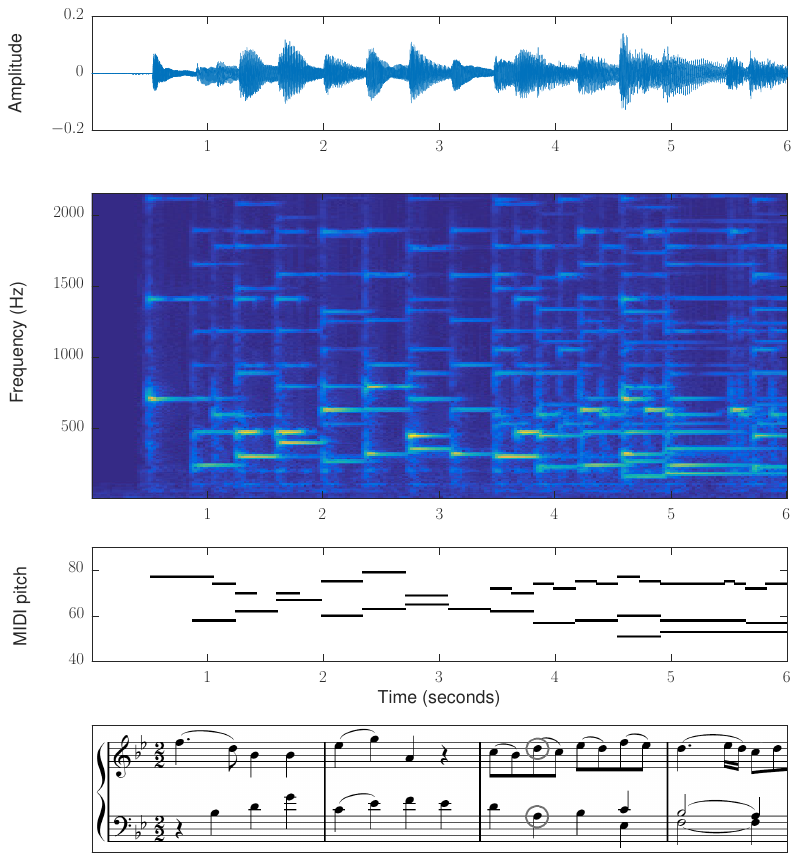
\includegraphics[width=12cm]{./statics/atm_data.png}
    \caption{نمایش‌های استفاده شده در یک سیستم \gls{ATM}.}
\end{figure}

در ادامه تلاش می‌شود به صورت مفصل‌تر به اهمیت و چالش‌های این مسئله پرداخته شود.

\subsection{کاربردها و تاثیرات}
یک سیستم \gls{atm} که بتواند به درستی کار کند، می‌تواند کاربردهای گسترده‌ای
همانند آموزش موسیقی، تولید موسیقی‌های جدید، توزیع موسیقی، جست‌وجو موسیقی و
مطالعه موسیقی داشته باشد. در نتیجه \gls{ATM} را می‌تواند تکنولوژی تاثیرگذار با
منفعت اقتصادی و اجتماعی بالا دانست.

\gls{atm} به صورت مستقیم با مسائل پردازش سیگنالی همچون جداسازی منبع‌های صوتی
مرتبط هست که هدف آن استخراج یک صوت تولیدی یک منبع خاص در مجموعه‌ای از صوات ضبط
شده هست. همچنین با توجه به این که حل مسائل سطح بالایی همچنون تشخیص قطعات
بازنوازی شده و خوشه‌بندی قطعات موسیقی در حالت نوشتاری موسیقی بسیار ساده‌تر هست،
می‌توان یک سیستم \gls{ATM} را جزئی کلیدی برای حوزه \gls{mir} دانست. درنتیجه
\gls{ATM} حلقه اصلی ارتباط مسائل حوزه‌های پردازش سیگنال‌های موسیقی و پردازش
نمادین موسیقی هست.

باتوجه به تاثیر بلقوه یک سیستم \gls{atm}، علاوه بر تحقیقات آکادمیک، شرکت‌های
تجاری زیادی نیز به این مسئله علاقمه‌مند شده‌اند. برای نمونه می‌توان از
نرم‌افزارهایی همچون Melodyne، AudioScore، ScoreCloud و Transcribe یاد کرد. هرچند
با توجه به تفاوت هدف نهایی این نرم‌افزارها مقایسه مستقیم عملکرد این نرم‌افزارها
با تحقیقات انجام شده، مقایسه‌ای عادلانه نخواهد بود.

\subsection{ارتباط و شباهت با سایر مسائل}
\gls{atm} ارتباطی بسیار نزدیک با سایر مسائل پردازش سیگنال دارد. یک سیستم
\gls{ATM} را می‌توان معادل یک سیستم \gls{asr} در حوزه پردازش گفتار دانست. شباهت
این دو سیستم از این جهت هست که هر دو سیستم تلاش می‌کنند یک سیگنال صوتی را تبدیل
به حالت نوشتاری اطلاعات کنند. همچنین مانند \gls{cocktail party problem} در
پردازش گفتار، موسیقی معمولا شامل چندین صدای همزمان هست. ولی برخلاف گفتار این
صداها به شدت به هم وابسطه هستند. همچنین هر دوی سیستم‌های \gls{ATM}و \gls{ASR}
می‌توانند با استفاده از یک \gls{language model} که در کنار \gls{acoustic model} استفاده می‌شود،
می‌تواند دقت را افزایش دهند. همچنین با توجه به این موسیقی نیز مجموعه فواعد
دستوری مخصوص به خود دارد، ارتباطی مستقیم بین \gls{atm} و حوزه \gls{nlp} وجود
دارد \cite{boulanger2012modeling}.

در ادامه مسئله \gls{atm} با حوزه پردازش تصویر و بینایی ماشین نیز در ارتباط هست.
از آنجا که نمایش زمان-فرکانس مورد استفاده در این سیستم‌ها، یک نمایش دو بعدی هست،
می‌توان مسئله را به تشخیص نت‌ها در یک تصویر ورودی تقلیل داد. همچنین همانند اکثر
مسائل این حوزه که انسداد اجسام مورد مطالعه چالشی جدی هست، نت‌های موسیقی استفاده
شده در یک قطعه نیز، معمولا فضای تکسانی را در نمایش زمان-فرکانس مورد استفاده
اشغال می‌کنند.

\subsection{چالش‌ها}
در مقایسه با سایر مسائل حوزه پردازش سیگنال، چندین عامل باعث می‌شود تا مسئله
\gls{atm}، مسئله‌ای چالش‌برانگیز محسوب شود. موسیقی \gls{polyphonic} شامل چندین
منبع صوتی مختلف مانند ساز‌های مختلف و صدای خواننده هست. هر کدام از این منبع‌ها
قدرت صدا و \gls{timber} متفاوتی دارند. همچنین بعضی از این منابع صوتی می‌توانند
چندین نت را به صورت همزمان اجرا کنند. استنداج ویژگی‌های موسیقیایی همانند
\gls{pitch} در حجم از صداهای در هم تنیده، مسئله‌ای پیچیده محسوب می‌شود.

همچنین در یک قطعه موسیقی معمولا نت‌های استفاده با هم، دارای هارمونیک‌های یکسانی
نیز هستند. این همپوشانی هارمونیک‌ها مجددا باعث پیده‌تر شدن فرایند جداسازی
می‌شود. برای مثال یک آکورد دو ماژور را در نظر بگیرد. این آکورد شامل \gls{pitch}
های دو، می و سل می‌شود که فرکانس پایه آنها با هم نسبت ۴، ۵ و ۶ دارد. در نتیجه به
ترتیب ۴۶/۷, ۳۳/۳ و ۶۰ درصد هامونیک آن‌ها با هم همپوشانی دارد.

یکی دیگر از مشکلات، تبعیت زمان نت‌های موسیقیایی از ریتم و ساختار زمانی رایج در
موسیقی هست. برای مثال تلاش می‌شود که نت‌های مشابه زمان شروع و پایان یکسانی در
قطعات \gls{polyphonic} داشته باشند. این ارتباط زمانی نت‌ها با هم باعث می‌شود که
نتوان فرض مستقل بودن منابع صوتی مختلف را کرد که خود باعث پیچیده‌تر شدن جدا سازی
صوت‌های مختلف می‌شود.

مشکلی دیگر این مسئله پیچیدگی انجام این فرایند حتی توسط موسیقی‌دانان با تجربه
هست. این پیدگی باعث می‌شود که گردآوری \gls{dataset} جامع قرایندی بسیار سخت و پر
از خطا باشد. حتی روش‌هایی مثل روش پیشنهاد شده در \cite{su2015escaping} نیاز به
نوازندگان خبره و پیش‌پردازش و پس‌پردازش سنگین دارد. همچنین قابل توجه هست که
\gls{sheet music} که قطعه از روی آن اجرا شده نیز نمی‌توان به عنوان یک برچسب قطعی
از داده استفاده شود. هر نوازنده با توجه به سلیقه خود ممکن است جاهایی از آهنگ را
تغییر دهد تا احساس مورد نظر را ایجاد کند. همچنین تشخیص این که هر نت متعلق به
کدام بازه زمانی سیگنال صوتی است هم به هیچ وجه کاری بدیهی محسوب نمی‌شود. در نتیجه
حتی در صورت وجود \gls{sheet music} قطعه، در بهترین حالت می‌توان آن را برچسبی
ضعیف برای سیگنال صوتی فرض کرد.

چالش‌های مطرح شده معمولا تمامشان در سیستم‌های کنونی کامل حل نمی‌شوند که منجر به
خطایی همچون نت‌های اضافه یا کم، اکتاوهای اشتباه، نت‌های ترکیب شده یا تجزیه شده و
زمان شروع و پایان اشتباه می‌شود.
\chapter{بررسی کارهای مرتبط}
در طی چهار دهه گذشته روش‌های گوناگونی برای مسئله \gls{atm} پیشنهاد داده شده است.
با وجود این که هدف نهایی هر سیستم \gls{ATM} استخراج حالت نوشتاری موسیقی از روی
سیگنال‌های صوتی هست ولی اکثر راه‌حل‌های موجود تلاش می‌کند با رسید به یک هدف
میانی مسئله را حل کنند. با توجه به ماهیت این هدف‌های میانی و ساختار آن‌ها
می‌توان این روش‌ها را به چهار دسته کلی تقسیم کرد:
\begin{itemize}
    \item در سطح فرم
    \item در سطح نت
    \item در سطح جریان
    \item در سطح نماد
\end{itemize}

آوانویسی در سطح فرم یا \gls{mpe}، تخمین تعداد و \gls{pitch} نت‌های موجود در هر
یک فرم زمانی است. این فرم‌ها معمولا طولی در حدود چند میلی ثانیه دارند. هرچند این
تخمین معمولا برای هر فرم به صورت جدا انجام می‌شود ولی اطلاعات زمینه‌ای معمولا در
یک مرحله‌ پس‌پردازیش برای روی نتیجه به دست آمده اعمال می‌شوند تا دقت را افزایش
دهند. روش‌هایی که در سطح فرم تلاش می‌کنند که آوانسی را انجام دهند از مفهوم نت
استفاده‌ای نمی‌کنند و معمولا با هیچ فهموم موسیقیایی درگیر نمی‌شود.

حجم زیادی از روش‌های موجود در سطح فرم کار می‌کنند. روش‌هایی مانند پردازش سیگنال
به صورت سنتی \cite{emiya2009multipitch,su2015combining}، مدل‌های برپایه احتمال
\cite{duan2010multiple}، روش‌های برپایه بیز \cite{peeling2009generative}، \gls{nmf}
\cite{smaragdis2003non,vincent2009adaptive,benetos2013automatic,fuentes2013harmonic}
و روش‌های برپایه \gls{nn} \cite{sigtia2016end,kelz2016potential}. تمام این
روش‌ها نقاط قوت و ضعف خود را دارند و هنوز روشی به عنوان روش واحد انتخاب نشده
است. برای مثال روش‌های بر پایه پردازش سیگنال ساده‌تر و سریع‌تر هستند و قابلیت
تعمیم بالاتری به سازهای مختلف دارند. در حالی که روش‌های بر پایه \gls{dl} بر روی
یک ساز خاص، مثلا پیانو، به نتایج بهتری دست یافته‌اند. روش‌های بیضی می‌توانند
مدل‌سازی کاملی از فرآیند تولید صوت ارائه دهند، در حالی که به شدت پیچیده‌تر و
کندتر هستند.

آوانویسی در سطح نت، یک مرحله از \gls{MPE} سطح بالاتر هست از این جهت که این
روش‌ها فقط وجود یا عدم وجود نت در یک فرم را بررسی نمی‌کنند، بلکه فرم‌ها را به هم
وصل کرده و نت‌ها را در طول زمان بررسی می‌کنند. در \gls{ATM} معمولا هر نت را با
سه ویژگی \gls{pitch}، onset و offset مشخص می‌کنند \cite{klapuri2007signal}. با
توجه مبهم بودن offset در نت، در بعضی از سیستم‌ها، معمولا در نظر گرفته نمی‌شود.
در نتیجه مدل فقط \gls{pitch} و onset را پیشبینی می‌کنند.

حجم زیادی از روش‌های در سطح نت معمولا پس‌پردازیش‌هایی بر روی خروجی یک سیستم
\gls{MPE} هستند. به عنوان روش‌های استفاده شده می‌توان از \gls{hmm}
\cite{nam2011classification} و \gls{nn} \cite{boulanger2012modeling} نام برد. در
پس‌پردازیش‌های انجام شده معمولا هر نمونه به صورت جدا بررسی می‌شود و رابطه بین
نت‌ها همزمان در نظر گرفته نمی‌شود که باعث تشخیص اضافه یا کمتر نت‌هایی می‌شود که
هارمونیک مشترک با نت‌های درست دارند. از این جهت روش‌هایی بر پایه مدل موسیقی
پیشنهاد شده است تا در ارتباط بین نت‌ها نیز در نظر گرفته شود
\cite{boulanger2012modeling, sigtia2016end}. بخش دیگری از روش‌ها نت‌ها را مستقیم
از روی سیگنال صوت استخراج می‌کنند. برخی دیگر ابتدا onset هر نت را پیدا می‌کنند و
سپس \gls{pitch} را بین آن‌ها تشخیص می‌دهند \cite{marolt2004connectionist}. برخی
دیگر حتی کل اطلاعات را با هم استخراج می‌کنند
\cite{cogliati2016context,ewert2016piano,hawthorne2017onsets}.

آوانویسی در سطح جریان یا \gls{mps} هدفش گروه بندی نت‌ها تخمین زده شده در
مجموعه‌ای جریان هست که هر جریان معمولا متناظر با یک ساز هست. این گروه از روش‌ها
ارتباط نزدیکی با \gls{iss} دارد. یکی از مزایای \gls{MPS} نسب به روش‌های قبلی
بررسی و تاثیر دادن \gls{timber} است. کارهای انجام شده در این سطح بسیار محدود
هستند.

تمام سه روش توضیح داده شده خروجی اصطلاحا پارامتری دارند. علت این نامگذاری این
هست که این آوانویسی انجام شده، یکی از پارامترهایش سیگنال صوتی ورودی هست. این
آوانویسی‌ها با وجود این که تا حدی از مفاهیم مسیقیایی استفاده می‌کنند ولی خروجی
آن‌ها هنوز اختلاف زیادی با سطح مجردسازی انجام شده در \gls{sheet music} دارد.
مهمترین این اختلاف‌ها زمان هست که در هر سه روش در واحد ثانیه اندازه گرفته
می‌شود. در حالی که در موسیقی زمان در واحد ضرب اندازه گرفته می‌شود. همچنین
\gls{pitch} در فراکنس هست در حالی که در موسیقی معمولا هر نت نامی مانند دو مینور
دارد و باتوجه به گام قطعه تعریف می‌شود. در نهایت مفاهیمی مانند میزان، ضرب آهنگ،
تمپو، گام و هارمونی کاملا حذف شده‌اند.

هدف آوانویسی در سطح نماد این هست که خروجی سیستم، نمادگذاری قابل لمس برای انسان
باشد که تمام اطلاعات موسیقیایی لازم را در بردارد. خروجی مانند \gls{sheet music}.
آوانویسی در این سطح نیاز به درک عمیق مفاهیم موسیقی مانند هارمونیک و ریتم دارد.
ساختارهای هارمونیک مانند گام و آکوردها باعث تغییر شکل نمایش \gls{pitch} می‌شوند.
ساختارهای ریتمیک مثل ضرب و میزان باعث می‌شود که طول نت‌ها از ثانیه مستقل شود.

چندین مطالعه تلاش کرده‌اند که ساختارهای موسیقیایی رو از روی سیگنال صوتی یا
\gls{MIDI} به دست آید انجام شده است. با این وجود مطالاعات خیلی کمی برای روی یک
سیستم آوانویسی کامل انجام شده است که از این مفاهیم استفاده کند.

با این وجود که روش‌های بسیار متفاوتی برای \gls{atm} وجود دارد ولی در دهه گذشته
بهترین دقت به دست آمده از دو خانواده از روش‌ها بوده است:
\begin{itemize}
    \item \gls{nmf}
    \item \gls{nn}
\end{itemize}
هر دو خانواده این مسائل برای مسائل بسیار متفاوتی مانند پردازش گفتار، پردازش
تصویر و سیستم‌های پیشنهاددهنده استفاده شده‌اند و نتایج بسیار رضایت بخشی به دست
آورده‌اند. در ادامه استفاده هر دو روش برای سیستم‌های \gls{ATM} بررسی می‌شود.

\section{روش‌های برپایه‌ی \gls{nn}}
همانند دیگر مسائل مرتبط با حوزه تشخیص الگو، شبکه‌های عصبی تاثیر قابل توجهی بر
روی مسئله \gls{atm} و به صورت کلی‌تر حوزه \gls{mir} داشته‌اند. \gls{nn} توانایی
یادگیری توابع غیرخطی پیچیده‌ را دارند که به آن‌ها برای حل مسائل کمک می‌کند. با
این وجود در مقایسه با حوزه‌ای مانند بینایی ماشین، سرعت رشد استفاده از \gls{nn}
برای حل مسئله \gls{atm} پایین بوده است. در ادامه تلاش می‌کنیم چند علت این موضوع
را بررسی کنیم.

یکی از اولین استفاده‌ها از \gls{nn} برای حل مسئله توسط
\cite{marolt2004connectionist} ارائه شده است. بخش اصلی این مدل استفاده از شبکه
تاخیر زمانی بوده است که همانند یک \gls{cnn} در بعد زمان عمل می‌کند. هر چند
انتشار این روش به ۲۰۰۱ برمی‌گردد ولی همچنان روشی موثر محسوب می‌شود و روش‌های
جدیدتر خود را با آن مقایسه می‌کنند.

یک روش نسبت جدیدتر \cite{bock2012polyphonic} استفاده از دو \gls{spec} به عنوان
ورودی است. یک از این \glspl{spec} دقت بالاتری در بعد زمان دارند که که برای تشخیص
شروع نت‌ها از آن استفاده می‌شود. \gls{spec} دیگر دقت بالایی در بعد فرکانس دارد.
از این دقت بالاتر برای تشخیص نت‌های با فراکنس پایین‌تر استفاده می‌شود. این
ورودی‌ها به یک شبکه چند لایه با ساتختار \gls{lstm} داده می‌شوند. این استفاده از
\gls{LSTM} دو مزیت دارد. اولین خوبی این است که تغییرات هر نت در طول \gls{spec}
مشخص است و این شبکه به خوبی می‌تواند این تغییرات را مدل کند. حسن دیگر این است که
این شبکه می‌تواند روابط طولانی مدت بین نت‌ها را نیز فرا بگیرد. برای مثلا شبکه
می‌تواند یاد بگیرد که پس از دو نت اول یک آکورد، دو و سل، وجود نت سوم آکورد، فا،
محتمل هست. ولی صحت یادگرفتن این رابطه‌ها بین نت‌ها بررسی نشد.

در \cite{sigtia2016end} تلاش شد که این ارتباط بین نت‌ها با استفاده از یک مدل
موسیقیایی در کنار مدل صوتی مدل شود. از این روش در سیستم‌های \gls{asr} استفاده
می‌شود و تاثیر به سزایی دارد. برای ساخت مدل موسیقیایی اطلاعات نت‌های هر قطعه به
یک \gls{rnn} داده می‌شود تا بتواند پیشبینی کند در فرم بعدی چه نت‌هایی فعال خواهد
بود. ایراد این روش این است که مدل نیاز دارد که یک توزیع احتمالی بزرگ را یاد
بگیرد و استفاده کند. این توزیع، توزیع متناظر به فعال یا غیرفعال بودن هر کلاویه
پیانو هست که $2^{88}$ حالت دارد. برای مدلسازی این فضای احتمالی به این بزرگی، از
یک ساختار خیلی خاص استفاده شده است که این احتمال را به شکل دنباله‌ای از ضرب
احتمال‌های شرطی نشان می‌دهند. با این وجود، شبکه بهبود کمی نسبت به یک \gls{hmm}
نشان داد، که مجددا باعث شک در توانایی مدل‌سازی این ارتباطات می‌شود.

همچنین در \cite{kelz2016potential} با تمرکز تنها بر روی \gls{acoustic model}، و
تنظیم درست پارامترهای شبکه، باعث شد که دقت با اخلافی قابل توجه از افزایش پیدا
کند. با این وجود که استفاده از یک \gls{language model} در یک سیستم \gls{ASR}
باعث افزایش دقت به شکل محسوس می‌شود، شواهدی مشابه از مزیت این مدل‌ها در
\gls{ATM} هنوز به دست نیامده است.
\chapter{مروری بر مفاهیم مورد نیاز}
\section{تبدیلات سیگنال صوتی}
یک اجرای موسیقی می‌تواند کاملا توسط تغییرات ایجاد شده در فشار هوا طی زمان توصیف
شود. این نمایش به صورت سنتی محور افقی نماینده زمان است و محور عمودی نماینده
تغییرات ایجاد شده در فشار یا شدت سیگنال است. با توجه به این که کامپیوترها
توانایی پردازش اطلاعت پیوسته را ندارند، این سیگنال‌ها نیاز دارند تا گسسته‌سازی
شوند. با توجه به این گوش انسان می‌تواند اصواتی با فرکانس تا ۲۰ کیلوهرتز را بشنود
و پردازش کند، برای این که تمام اطلاعات مورد نیاز بتواند ذخیره شود، نمونه برداری
با حداقل دقت ۴۰ کیلوهرتز انجام شود. به صورت رایج موسیقی معمولا در ۴۴/۱ کیلوهرتز
نمونه برداری می‌شود. همچنین برای ذخیره هر نمونه از ۱۶ بیت استفاده می‌شود.
فایل‌های wav از این نمایش برای ذخیره سازی موسیقی استفاده می‌کنند.

هر چند که صوت تنها حاصل نوسانات ماده است، ولی سیستم شنوایی این نوسانات به
مجموعه‌ای از فرکانس‌ها تبدیل می‌شود و سپس پردازش می‌شوند. برای تشخیص میزان وجود
یک فرکانس خاص در یک سیگنال صوتی می‌توان همبستگی سیگنال صوتی را با یک سیگنال
سینوسی در فرکانس خواسته شده را محاسبه کرد. هرچند دو سیگنال سینوسی با فرکانس
یک‌سان نیز می‌توانند همبستگی صفر داشته باشند اگر فاز آن‌ها به میزان مناسبی با هم
اختلاف داشته باشد. این موضوع به خوبی در شکل زیر نشان داده شده است.
\begin{figure}[ht]
    \centering
    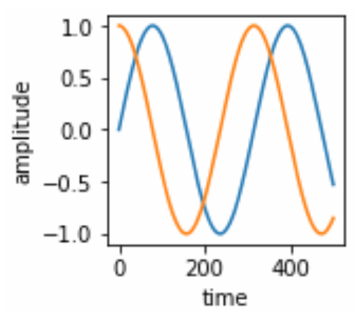
\includegraphics[height=5cm]{./statics/uncorrelated_sine_waves.png}
    \caption{دو سیگنال سینوسی که با هم وابستگی ندارند ولی هر دو در فرکانس یکسانی نوسان می‌کنند}
\end{figure}

برای اندازگیری همبستگی به ازای تمام فازهای ممکن، مانند فازی که باعث می‌شود تا
مقدار همبستگی حداکثر شود، از اعداد موهومی استفاده می‌شود. فرض کنید نقطه‌ای برروی
محور اعداد موهومی از مبدا و در جهت اعداد حقیقی مثبت شروع به حرکت کند. جهت حرکت
این نقطه با با توجه به فرکانس خواسته شده تغییر می‌کنند. همچنین سرعت حرکت این
نقطه در لحظه $t$ برابر با قدرت سیگنال ورودی در  لحظه $t$ است. به عبارتی دیگر،
نقطه یاد شده در زمان $t$ به اندازه قدرت سیگنال ورودی در زمان $t$ و در جهت محاسبه
شده جابه‌جا می‌شود. در پایان فرآیند هرچه نقطه از مبدا دورتر شده باشد، یعنی
وابستگی سیگنال ورودی با سیگنالی سینوسی با فرکانسی برابر فرکانس خواسته شده بیشتر
است. همچنین فازی که باعث بیشتر مقدار وابستگی می‌شود، با جهت کلی حرکت در ارتباط
هست. شکل زیر نمونه‌ای از انجام این فرآیند را برای دو سیگنال مختلف نشان می‌دهد.
مطابق انتظار برای سیگنالی که هم بستگی بسیار پایینی با فرکانس خواسته شده دارد،
نقطه نزدیک مبدا است و برای سیگنالی که همبستگی بیشتری دارد، از مبدا دورتر است.
\begin{figure}[ht]
    \centering
    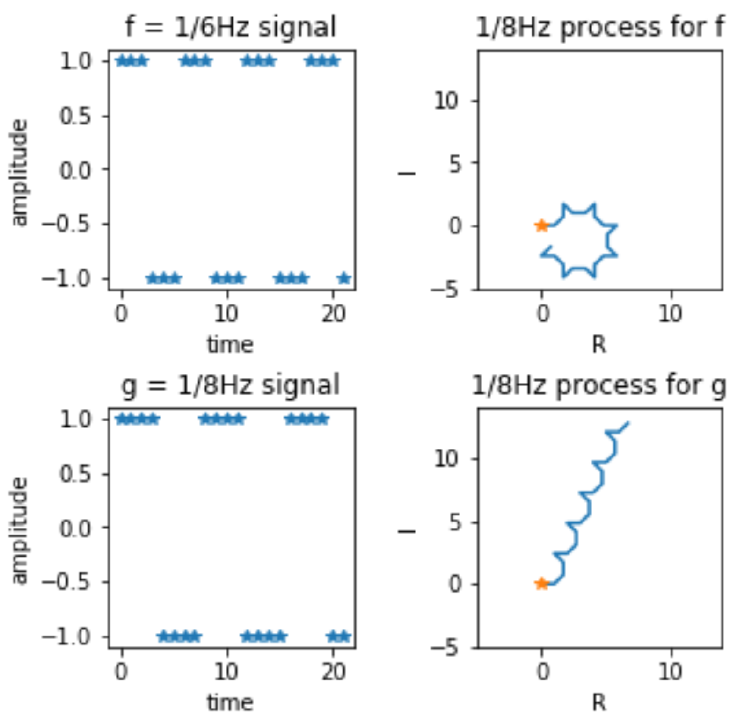
\includegraphics[height=8cm]{./statics/spectral_domain_process.png}
    \caption{انجام فرایند توضیح داده شد بر روی دو سیگنال ورودی مختلف}
\end{figure}

فرایند بالا را می‌توان توسط رابطه زیر مدل کرد:
\begin{equation}
    X(\omega) = \sum_{n} x(n)e^{i \omega \frac{2\pi}{f_s} n}
\end{equation}
که $X(\omega)$ عددی موهومی است که اندازه آن برابر است با میزان حضور یک فرکانس
دلخواه مانند $\omega$ در سیگنال ورودی $x$. همچنین $x(n)$ میزان قدرت سیگنال در در
نمونه $n$ نشان می‌دهد. $e^{i \omega \frac{2\pi}{f_s}}$ برابر جهت حرکت در محور‌
مختصات اعداد موهومی در زمان $t = \frac{n}{f_s}$ است که $f_s$ فرکانس خواسته شد
است. محل توقف نقطه در فرآیند یاد شده همان خروجی این رابطه است که اندازه آن با
میزان حضور فرکانس مطلوب در سیگنال ورودی رابطه دارد.

با کمک رابطه بالا می‌توان می‌توان میزان وجود هر فرکانس در سیگنال ورودی را اندازه
گرفت و در نتیجه سیگنال ورودی را به حوزه فرکانس انتقال داد. حوزه فرکانس میزان
قدرت هر فرکانس در سیگنال ورودی را بیان می‌کند در حالی که حوزه زمان که ابتدا سیگنال
در آن بود قدرت سیگنال در زمان‌های مختلف را مشخص می‌کند.

\subsection{تبدیل فوریه}
معروف‌ترین تبدیل برای انتقال سیگنال از حوزه زمان به حوزه فرکانس تبدیل فرویه هست.
\gls{fft} یک پیاده سازی از این تبدیل است که سیگنال‌هایی که طول آن‌ها توانی از دو
است را می‌توان در $O(nlog(n))$ به حوزه فرکانس ببرد. این تبدیل میزان فعال بودن
فرکانس‌های مختلف را که فاصله خطی از هم دارند را به گونه‌ای محاسبه می‌کند که
سیگنال ابتدایی مجدد بعد از تبدیل قابل محاسبه است. این تبدیل سیگنال ورودی را به
شکل حاصل جمع مجموعه‌ای موج سینوسی با فرکانس‌های مختلف بیان می‌کند. صورت گسسته
این تبدیل که به \gls{dft} معروف است توسط رابطه زیر قابل محاسبه است:
\begin{equation}
    X[k] = \sum_{n=0}^{N-1} x[n]e^{- ikw\omega_0n} \quad \forall k \in \{ 0, 1, ..., N-1 \}
\end{equation}
که $x$ سیگنال ورودی به طول $N$ است و $\omega_0$ برابر $\frac{2\pi}{n}$ است.

همچنین برای بازتولید سیگنال اولیه می‌توان از رابطه زیر استفاده کرد:
\begin{equation}
    x[n] = \frac{1}{N}\sum_{k=0}^{N-1} X[k]e^{ik\omega_0n} \quad \forall n \in \{ 0, 1, ..., N-1 \}
\end{equation}

به صورتی کلی وقتی خروجی تبدیل بررسی می‌شوند تنها اندازه اعداد موهومی به دست آمده
استفاده می‌شود. اندازه این اعداد متناسب با همبستگی سیگنال ورودی با سیگنال‌های
سینوسی بهینه است.

با توجه به سرعت \gls{fft} این تبدیل از حوزه‌های متفاوت به صورت گسترده استفاده
می‌شود. با این وجود در حوزه \gls{mir} این تبدیل یک ضعف مهم دارد. به کمک این
تبدیل می‌توان متوجه شد که یک فرکانس خاص، مثلا ۴۴۰ هرتز، در یک قطعه وجود دارد ولی
راهی برای تشخیص مکان وجود این فرکانس وجود ندارد. یک راه حل برای این ضعف این است
که سیگنال ورودی در فواصل کوتاه برش داده شود و برای هر برش به صورت جداگانه تبدیل
محاسبه گردد. این تبدیل جدید به \gls{stft} معروف است. هرچی فاصله زمانی که برش‌ها
در آن‌ها انجام می‌شود کوتاه‌تر باشد، دقت خروجی در بعد زمان بیشتر است. از طرفی
دیگر کوتاه بودن این فواصل زمانی باعث کاهش دقت در بعد فرکانس می‌شود. خروجی
\gls{STFT} یک نمایش دو بعدی است که یک محور آن نماینده زمان و محور دیگر نماینده
فرکانس است. این نمایش به نمایش زمان-فرکانس معروف است.

\subsection{تبدیل ثابت Q}
یکی از ضعف‌های \gls{stft} در حوزه موسیقی این است که فرکانس‌هایی که وجود آن‌ها در
سیگنال ورودی بررسی می‌شود، فاصله خطی از یک دیگر دارند. این در حالی هست که
\gls{pitch} نت‌های موسیقی در فواصل لگاریتمی از یک دیگر قرار دارند. این تفاوت‌ به
این معنی است که برای نت‌های بم تعداد زیادی فرکانس وجود دارد ولی برای نت‌های
زیرتر فرکانس‌های کمتری وجود دارد.

\gls{cqt} بجای استفاده از فواصل خطی از فواصل لگاریتمی استفاده می‌کند. ایده اصلی
این است که در فرایند توضیح داده شده در ابتدا، فرکانس‌های انتخابی، فاصله‌ای
لگاریتمی نسبت به هم داشته باشند. همچنین این تبدیل به کمک توابع پنجره‌بندی تنها
در بازه‌های زمانی خاصی، وجود فرکانس‌ها را بررسی می‌کند.
\begin{figure}
    \centering
    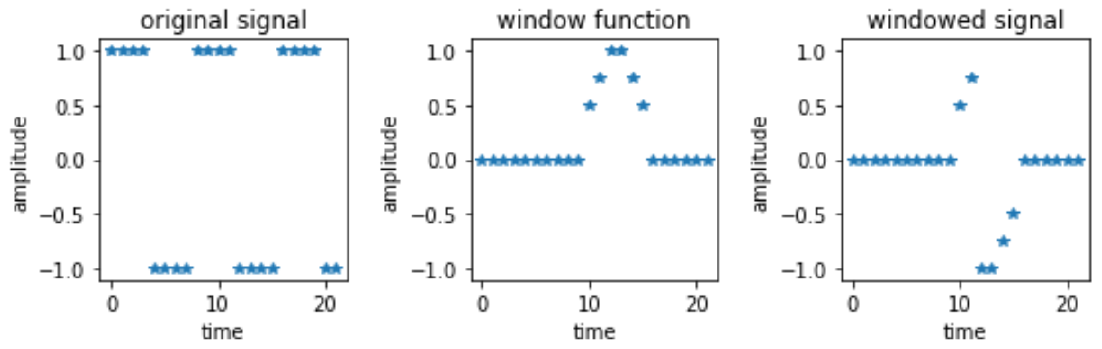
\includegraphics[height=4cm]{./statics/windowed_signal.png}
    \caption{نمونه‌ای از یک سیگنال پنجره‌بندی شده}
\end{figure}

\gls{CQT} را می‌توان به کمک رابطه زیر محاسبه کرد:
\begin{equation}
    X^{CQ}(k, n) = \sum_{j=n-\lfloor N_k / 2 \rfloor}^{n+\lfloor N_k / 2 \rfloor} x(j)a_k^*(j-n+N_k/2) \quad \forall k \in \{1, 2, ..., K \}
\end{equation}
\begin{equation}
    a_k^*(n) = \frac{1}{N_k} w (\frac{n}{N_k}) e^{if_k\frac{2\pi}{f_s}n}
\end{equation}
$X^{CQ}(k, n)$ مقدار خروجی تبدیل برای فرکانس $f_k$ و در اطراف نمونه $n$ سیگنال
ورودی $x$ است. $N_k$ یک عدد حقیقی هست که از پارامترهای تبدیل است. $w$ یک تابع
پنجره‌بندی پیوسته هست که دامنه آن بین صفر و یک است. $f_k$ فرکانس خواسته شده‌
$k$ام است. $f_s$ نیز فرکانسی است که سیگنال ورودی با آن نمونه برداری شده است.

این تبدیل پارامترهای مختلفی دارد که مقدار بهینه آن‌ها با توجه به معیار‌هایی
مانند توانایی باز تولید سیگنال و سرعت محاسبه در \cite{schorkhuber2010constant}
بررسی شده است. در ادامه به بررسی این پارامترها می‌پردازیم.

$f_k$ مقدار فرکانس $k$ام خواسته شده را مشخص می‌کند. با توجه به این که این
فرکانس‌ها با هم فاصله‌ای لگاریتمی دارند، می‌توان مقدار آن‌ها را مقایسه کرد. برای
محاسبه می‌توان از رابطه زیر استفاده کرد:
\begin{equation}
    f_k = f_1 2^{\frac{k-1}{B}} \quad \forall k \in \{1, 2, ..., K\}
\end{equation}
$f_1$ یا $f_{min}$ مقدار پایین‌ترین فرکانس را مشخص می‌کند که سایر فرکانس‌ها از
آن شروع می‌شوند. $B$ مشخص می‌کند به ازای هر اکتاو چند فرکانس انتخاب شود و میزان
حضور آن‌ها در سیگنال ورودی اندازه گرفته شود. همچنین $K$ تعداد کل فرکانس‌های
خواسته شده است. این مقدارها با توجه کاربرد به می‌توانند انتخاب شوند.

$N_k$ عرض پنجره استفاده شده برای فرکانس $k$ام را مشخص می‌کند. مقدار بهینه این
پارامتر را می‌توان با استفاده از رابطه زیر محاسبه کرد:
\begin{equation}
    N_k = \frac{qf_s}{f_k(2^{\frac{1}{b}}-1)} \stackrel{B \geq 12}{\approx} \frac{qf_sB}{log(2)f_k} \quad 0 < q \leq 1
\end{equation}

انجام \gls{cqt} برای هر نمونه نه از نظر محاسبه منطقی است و نه مزیت خاصی دارد. از
این جهت این تبدیل به ازای هر $H_k$ نمونه یک بار انجام می‌شود. مقدار بهینه برای
این پارامتر برابر $\lfloor \frac{1}{2N_k} \rfloor$ است تا تمام طول سیگنال ورودی
پردازش شود. همچنین در عمل معمولا به ازای تمام مقادیر $k$، $H_k = H$ است تا خروجی
را بتوان به شکل یک ماتریس نمایش داد.

$w$ تابع پنجره‌بندی مورد استفاده است که به صورت سنتی از تابع $Hann$ برای آن
استفاده می‌شود. این تابع برشی از تابع سینوس‌ هست که در زیر نمودار آن نشان داده شده
است.
\begin{figure}[ht]
    \centering
    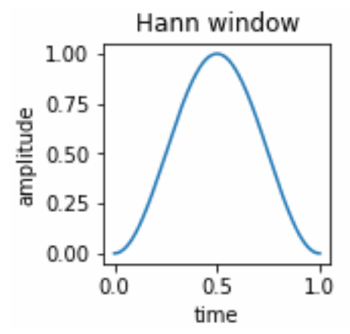
\includegraphics[height=5cm]{./statics/hann_plot.png}
    \caption{نمودار تابع پنجره‌بندی Hann}
\end{figure}

در نهایت $f_s$ فرکانس نمونه‌برداری از سیگنال اولیه است. برای صحت محاسبات رابطه
زیر باید برقرار باشد:
\begin{equation}
    f_s \geq 2f_k
\end{equation}

\subsection{اسپکتروگرام mel}
با توجه به این که درک انسان از صوت یک درک کاملا لگاریتمی نیست، مقیاس دیگری برای
انجام آزمایشات ساخته شده است که به مقیاس mel معروف است. با وجود این که بیش از یک
مقیاس mel ساخته شده، ولی تمام آن‌ها تنها تفاوت‌هایی جزئی با هم دارند. در این
پایان‌نامه فقط یکی از این مقیاس‌ها توضیح داده شده است که همان مقیاسی است که در
این پایان‌نامه استفاده شده است و کتابخانه librosa آن را پیاده‌سازی کرده است
\cite{mcfee2015librosa}.

آزمایشات انجام شده بر روی شنوایی انسان نشان داده‌اند که درک انسان از صوت، تا
هزار هرتز، یک درک خطی است. برای اصوات بالای هزار هرتز این درک به شکل لگاریتمی در
می‌آید. با این توصیف رابطه زیر می‌تواند این مقیاس را مدل کند:
\begin{equation}
    x Hz =
    \begin{cases}
        \frac{3x}{200}mel &\quad x \leq 1000\\
        15 + 27 ln(x/1000) / ln(6.4) mel &\quad \text{elsewhere}
    \end{cases}
\end{equation}

کتاب‌خانه librosa \gls{spec} با مقیاس mel را به کمک رابطه زیر محاسبه می‌کند:
\begin{equation}
    X^{MEL}(k, n) = \sum_{j=0}^{n_{fft}-1} |X_n|^2(j)A_k^*(\frac{f_s}{n_{fft}}j)
\end{equation}
$|X_n|$ اندازه \gls{dft} سیگنال ورودی $x$ در اطراف $n$ با $n_{fft}$ نمونه است.
$A_k^*$ یک تابع پنجره‌بندی از اعداد حقیقی به اعداد حقیقی است. این تابع شکلی
مثلثی دارد و در $f_{k-1}$ مقدار صفر دارد. در $f_k$ به $V_{max}^{k}$ می‌رسد و
مجددا در $f_{k+1}$ صفر می‌شود. $V_{max}^{k}$ به گونه‌ای مقدار داده می‌شود که
تقریبا برای هر کانال مقداری ثابت داشته باشد. این مقدار از رابطه زیر به دست
می‌آید:
\begin{equation}
    V_{max}^{k} = \frac{2}{f_{k+1} - f_{k-1}}
\end{equation}
$\frac{f_s}{n_{fft}}j$ فرکانس متناظر با $j$امین فرکانس استفاده شده در \gls{dft}
است. همچنین $f_s$ فرکانس نمونه‌گیری سیگنال ورودی $x$ است.

\subsection{قالب فرکانسی یک نت}
وقتی که صوت حاصل از اجرای یک نت تنها، از حوزه زمان به خوزه فرکانس انتقال داده
شود، \gls{spec} به دست آمده، قالب فرکانس آن نت نامیده می‌شود. وقتی که

در شکل زیر قالب فرکانسی نت $A5$ که بر روی ساز پیانو اجرا شده است رسم شده است.
همچنین فرکانس‌ها با یک دیگر فاصله‌ای لگاریتمی دارند تا متناظر با \gls{pitch}
نت‌های پیانو باشند. همچنین که در \gls{spec} رسم شده کاملا واضح است، علاوه بر
فرکانس پایه نت، فرکانس‌های پایه‌ای دیگری نیز کامل در صوت تولید شده حضور دارند.
این فرکانس‌ها با خط سفید مشخص شده‌اند. این پدیده رفتاری کاملا انتظار از یک ساز
موسیقی است و یکی از عوامل اصلی سختی مسئله \gls{atm} محسوب می‌شود. همچنین این
رفتار وجه اصلی تمایز مسئله \gls{asr} با مسئله \gls{atm} است. این فرکانس‌‌های
فعال، به عنوان هامونیک‌های نت نواخته شده شناخته می‌شود. با توجه به این که این
هامونیک‌ها خود متناظر با نت‌های دیگری نیز هستند که احتمال نواخته شدن بالایی نیز
با نت پایه دارند، تشخیص نت‌های فعال را بسیار پیچیده می‌کنند.

همچنین، با توجه به شکل کاملا واضح است که در لظحه نواخته شدن نت، فرکانس‌های فعال
دیگری نیز در صوت تولید شده حضور دارند. دلیل حضور این فرکانس‌ها این است که وقتی
یک سیم پیانو توسط چکش نواخته می‌شود، در لحظه شروع حجم زیادی نویز تولید می‌کند که
باعث حضور بازه گسترده‌ای از فرکانس‌ها می‌شود. ولی پس از گذشت زمانی کوتاه، سیم
شروع می‌کند به در فرکانس متناظر نوسان کردن و فرکانس‌های اضافه حذف می‌شوند. حضور
این بازه گسترده از فرکانس‌ها باعث می‌شود که شروع نت‌ها به شکل بسیار ساده‌تری
قابل تشخیص باشد.
\begin{figure}[ht]
    \centering
    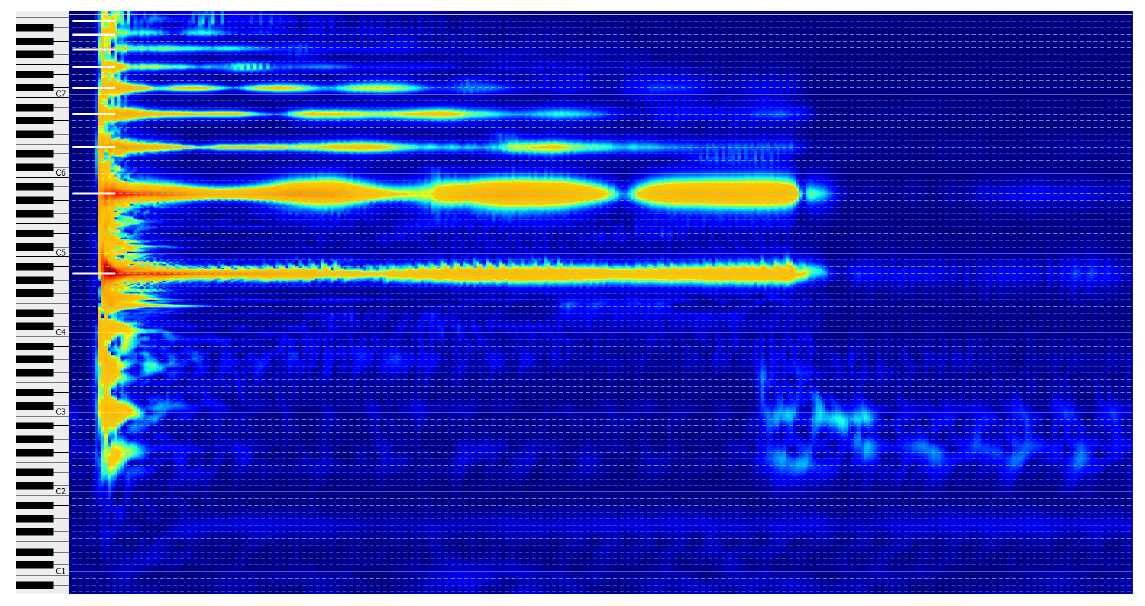
\includegraphics[width=15cm]{./statics/a5_spec.png}
    \caption{\gls{spec} متناظر با نواخته شدن نت A5 بر روی پیانو}
\end{figure}

\section{یادگیری ژرف}
در سال‌های اخیر، \gls{ml} روز به روز محبوب‌تر شده‌است در برای حل مسائلی مانند
دسته‌بندی تصاویر، پیشنهاد ویدیو، تحلیل شبکه‌های اجتماعی و پردازش متن به صورت
گسترده استفاده می‌شود. در میان روش‌های \gls{ml}، \gls{dl} موفقیت‌های بسیاری برای
حل این مسائل و مسائل دیگر به دست آورده است. رشد نمایی داده و پیشرفت‌های
سخت‌افزاری باعث شده که تحقیقات گسترده‌ای بر روی \gls{dl} صورت بپذیرد. \gls{dl}
که پیدایش آن ریشه در \gls{nn} دارد، توانسته به خوبی از پدران خود پیشه بگیرد و
نتایج بسیاری بهتری به دست بیاورد. روش‌های اخیر در \gls{dl} نتایج بسیار امیدوار
کننده‌ای در حوزه‌های پردازش تصویر، گفتار و زبان طبیعی به دست آورده‌اند و در خیلی
از مسائل انسان حتی پیشه گرفته‌اند.

به صورت سنتی، نمایشی که برای برای داده انتخاب می‌شود، تاثیر به سزایی در دقت
نهایی سیستم دارد و یک نمایش نامناسب از داده باعث دقت به‌شدت پایین‌تری می‌شده
است. از این جهت بررسی شیوه‌های موثر نمایش داده، در \gls{ml}، از چالش‌های اصلی
حوزه محسوب می‌شده است و مطالعات زیادی بر روی آن‌ها انجام شده است. با این وجود
این یافته‌ها اکثرا تنها محدود به حوزه خاصی هستند و قابل تعمیم به سایر حوزه‌ها
نیستند.

در مقابل، در \gls{dl}، تمام این فرایند استخراج ویژگی از داده‌های ورودی و تبدیل
آن‌ها به نمایشی مناسب، به صورت خوکار، توسط مدل فراگرفته و اعمال می‌شود. این
ویژگی این خانواده از مدل‌ها باعث می‌شود که نیاز به دخالت متخصص حداقل شود و
سیستم‌هایی کارا، بدون نیاز دانش حوزه، طراحی شوند.

سیستم‌های مبتنی بر \gls{dl} شامل مجموعه‌ای از لایه‌های غیرخطی هستند که می‌توانند
اطلاعات را در ساختاری سلسله‌مراتبی استخراج کنند. لایه‌های ابتدایی مدل، مسئول
استخراج ویژگی‌های سطح پایین‌تر هستند. سپس لایه‌های بعدی از این ویژگی‌های استخراج
شده استفاده می‌کنند تا ویژگی‌های سطح بالاتری را استخراج کنند. این دقیقا همان
رفتاری است که مغز انسان برای پردازش داده‌های ورودی و تصمیم‌گیری بر اساس آن‌ها
انجام می‌دهد. برای مثال در سیستم بینایی انسان، نرون‌های ابتدایی تنها وظیفه
استخراج نقطه‌ها را دارند. از موقعیت نقطه‌های استخراج شده استفاده می‌شود تا خطوط
تشخیص داده شوند. به همین شکل مغز اشکال پیچیده‌تر را پیدا می‌کند و تشخیص می‌دهد
در لحظه در حال مشاهده چه اجسامی می‌باشد.

\subsection{تاریخچه یادگیری ژرف}
ساختن ماشینی که مشابه مغز انسان کار کند و بتواند مانند مغز مسائل را حل کند
رویایی به قدمت چندین قرن برای دانشمندان است با این حال شروع تاریخجه مدرن
\gls{dl} را می‌توان از ۱۹۴۳ دانست که \lr{McCulloch-Pitts} معرفی شد. این مدل
اولین مدل ساختار نرون محسوب می‌شود و نمونه‌ای اولیه از \gls{nn} امروزی است. مدل
معرفی شده می‌توانست تا حدی رفتار یک نرون مغزی را مدل کند ولی هیچ قاعده‌ای برای
یادگیری معرفی شد. از آن زمان \gls{dl} به آرامی شروع به پیداش و پیشرفت کرد و طی
چندین رخداد مهم تبدیل به ساختار امروزی شد.

پس از معرفی مدل \lr{McCulloch-Pitts} قاعده یادگیری هب معرفی شد که ریشه‌ای زیستی
دارد و برای آموزش شبکه‌های اولیه استفاده می‌شود. سپس در سال ۱۹۵۸ در حوزه علوم
شناختی، مدل پرسپترون معرفی شد که ساختاری بسیار نزدیک به \gls{nn} امروزی دارد. با
پایان یافتن دوره رکود اولی \gls{ai}، پیدایش \gls{backpropagation} رخداد تارخی
مهم بعدی در پیدایش \gls{dl} بود. به کمک \gls{backpropagation} آموزش \gls{nn} به
کمک یک تابع خطا ممکن شد. در سال ۱۹۸۰ neocogitron معرفی شد که منجر به پیدایش
\gls{cnn} شد. همچنین در سال ۱۹۸۶ با معرفی \gls{rnn} امکان پردازش داده‌های
دنباله‌ای محقق شد. در نهایت در ده ۹۰ میلادی با معرفی LeNet اولین شبکه عصبی عمیق
معرفی شد. هرچند این شبکه در زمان انتشار، به علت محدودیت‌های سخت‌افزاری به شهرت
زیادی دست نیافت.

در ۲۰۰۶ \gls{dbn} همراه با یک شیوه آموزش لایه به لایه معرفی شدند. ایده اصلی این
شبکه‌ها این بود که یک شبکه دولایه ساده با \gls{unsupervised learning} و مشابه
\gls{rbm} آموزش داده شود. سپس تمام پارامترهای فراگرفته شده قفل شوند، یک لایه
جدید در ادامه شبکه قرار داده شود، و پارامترهای این لایه همچون لایه قبل فراگرفته
شود. با کمک این شیوه آموزش، محققان توانستند شبکه‌هایی با عمق به شدت بیشتر از
مدل‌های قبلی را آموزش دهند. \gls{dl} بعد از سال‌ها توسعه و با ریشه در \gls{nn}
یکی از روش‌های پرطرفدار در \gls{ml} محسوب می‌شوند که توانسته است موفقیت‌های
زیادی به دست آورد.

از موفقیت‌های اخیر \gls{dl} می‌توان از AlphaGo نام برد که در ابتدای ۲۰۱۷ توسط
تیمی از گوگل معرفی شد و با عملکرد خود دنیا را متعجب ساخت. این مدل توانست تحت نام
مستعار master، ۶۰ بازی Go در مقابل حریفان حرفه‌ای برنده شود. از جمله این
پیروزی‌ها سه برد پیاپی در مقابل \lr{Ke Jie} است. این شبکه توانست با بهره‌گیری از
روش‌های مدرن \gls{dl} و سخت‌افزاری قدرتمند برای آموزش، قهرمان چهانی این بازی را
شکست دهد.

\subsection{شبکه‌های عصبی مصنوعی}
شبکه‌های عصبی مصنوعی سیستم‌های محاسباتی هستند که از شبکه‌های عصبی زیستی الهام
گرفته‌اند. این سیستم‌ها از طریق مشاهده مثال‌ها و بدون نیاز به برنامه‌ریزی مستقیم
می‌توانند مسائل مختلفی را حل کنند. برای مثال این شبکه‌ها با دیدن تصاویر زیادی که
حاوی ماشین بوده‌اند، در تصاویر جدید ماشین را، بدون نیاز به تعریف مستقیم ماشین،
تشخیص دهند. از این جهت از شبکه‌های عصبی مصنوعی در حل مسائلی که نمی‌توان به راحتی
از طریق الگوریتم‌های قانونمند برای حل آن‌ها اقدام کرد، استفاده می‌شود.

یک شبکه عصبی مصنوعی از تعداد زیادی واحدهای کوچک‌تر که یک نرون مصنوعی نامیده
می‌شوند تشکیل شده است. این نرون‌ها توسط اتصالاتی به نام سیناپس به یکدیگر مرتبط
اند که می‌تواند سیگنال‌ها را از نرونی به نرون بعدی منتقل کند. به این طریق هر
نرون می‌تواند مجموعه‌ای از سیگنال‌های ورودی را گرفته، آن‌ها را پردازش کند و از
طریق سیگنالی نتیجه را به نرون‌های بعدی منتقل کند. همچنین این سیناپس‌ها معمولا
دارای وزن‌هایی می‌باشند که میزان اهمیت یک سیگنال برای نرون دریافت کننده آن را
نشان می‌دهد و فرآیند یادگیری شامل تنظیم این وزن‌ها است.

به طور معمول نرون‌ها به شکل لایه لایه قرار داده می‌شنود که هر لایه عمل مخصوص به
خود را انجام می‌دهد و نتیجه را به لایه بعد منتقل می‌کند. برای مثال شبکه‌ای را در
نظر بگیرید که هدف آن تشخیص اشیای مختلف باشد. این شبکه از لایه‌های مختلفی تشکیل
شده است. در فرآیند یادگیری ممکن است این لایه اول نسبت به خطها حساس شده باشد.
یعنی هر نرون این لایه در صورت وجود خطی با زاویه و ضخامتی مشخص و در جایی مشخص از
تصویر، سیگنال‌های شدیدتری به لایه بعدی ارسال کند. حال لایه بعد می‌تواند از
اطلاعات ارسالی از لایه قبل استفاده کرده، و با توجه به اطلاعات خطها شکل‌های هندسی
ساده را تشخیص دهد.

هدف اصلی شبکه‌های عصبی مصنوعی پردازش اطلاعات و حل مسائل به همان شیوه‌ای بود که
مغز انسان مسائل را حل می‌کند. ولی در طول زمان با تمرکز بروی مسائل مختلف باعث شد
عملکردهایی اضافه شوند که گاها هیچ توجیح زیستی‌ای ندارند. به عنوان نمونه می‌توان
به فرآیند پس‌انتشار خطا اشاره کرد که با این که هیچ ریشه زیستی ندارند ولی یکی از
اصلی‌ترین شیوه‌های آموزش شبکه‌های عصبی عمیق محسوب می‌شود.

با گذر زمان و افزایش توان محاسباتی کامپیوترها، دانشمندان توانستند شبکه‌های عصبی
بزرگ‌تر و پیچیده‌تری طراحی کنند و با استفاده از آن‌ها مسائل سخت‌تری را حل
نمایند. در حال حاضر هر شبکه ممکن است تا حدود چند میلیون نرون داشته باشد. با این
حال هنوز تا شبکه‌هایی به پیچیدگی مغز انسان که راه بسیاری باقی مانده است.

\subsection{روش‌های یادگیری}
روش‌های \gls{dl} را می‌توان به سه دسته \gls{supervised learning}،
\gls{unsupervised learning} و \gls{semisupervised learning} تقسیم کرد. همچنین
\gls{reinforcement learning} نیز دسته دیگری از روش‌ها را شامل می‌شود که خود زیر مجموعه‌ای از
روش‌های \gls{semisupervised learning} است.

\gls{supervised learning} روش‌هایی هستند که از برچسب داده‌گان برای آموزش استفاده
می‌کنند. در این خانواده از روش‌ها دادگان به شکل زوج مرتب $(x, y)$ هستند که $x$
ورودی مدل است و $y$ خروجی مورد نظر است. در صورتی که مدل به ازای ورودی $x$ مقدار
$y^{\prime}$ را برگداند، مقادیر $y$ و $y^\prime$ به یک تابع خطا، مثلا $L$، داده
می‌شوند و پارامترهای مدل به گونه‌ای تغییر داده می‌شود که مقدار $L(y, y^\prime)$
کاهش یابد. پس از پایان آموزش انتظار می‌رد که در صورتی که ورودی $x$ به مدل داده
شود، مدل بتواند جواب درست، $y$ را تشخیص دهد و برگرداند.

\gls{unsupervised learning} به روش‌هایی گفته می‌شود که داده‌گان مورد آموزش در
آن‌ها دارای برچسب نمی‌باشد. در این روش‌ها مدل تلاش می‌کند تا ساختار داخلی یا
ویژگی‌های مهم ورودی را فراگیرد و با کمک آن‌ها روابط بین داده‌گان ورودی را
پیدا کند. \gls{clustering} و \gls{dimensionality reduction} نمونه‌هایی از مسائل
\gls{unsupervised learning} محسوب می‌شوند.

\gls{semisupervised learning} به روش‌هایی اطلاق می‌شود که تنها بخشی از دادگان
آموزش آن‌ها دارای برچسب هستند. در این روش‌ها معمولا بخشی از مدل توسط روش‌های
\gls{unsupervised learning} و بخش دیگر توسط روش‌های \gls{supervised learning}
آموزش داده می‌شود.

\subsection{طراحی و آموزش شبکه‌ها عصبی عمیق}
طراحی شبکه‌های عصبی شامل تعیین تعداد لایه‌ها، نوع و اندازه هر لایه، شیوه ارتباط
لایه‌ها و تابع خطا با توجه ماهیت مسئله مورد نظر است. این پارامترها که ساختار مدل
را مشخص می‌کنند با نام \gls{hyper parameter} شناخته می‌شوند.

فرض کنید یک شبکه عصبی یک تابع هست که می‌خواهد تقریبی از تابع $f$ از $X$ به $Y$
باشد. نمونه‌هایی از مقادیر $X$ و مقدار متناظر آن‌ها در $Y$ به شکل \gls{dataset}
آموزش داده شده‌اند. ساختار استفاده شده برای شبکه، شکل این تابع مشخص می‌کند و
محدودیتی بر روی ساختار آن اعمال می‌کند. از این جهت در زمان طراحی تلاش می‌شود تا
ساختار به گونه‌ای انتخاب شود که محدودیت‌های اعمال شده مانع انعطاف پذیری مورد
نیاز تابع نشوند و تابع ظرفیت کافی برای تقریبی مناسب را دارا باشد. همچنین تابع
انعطاف پذیری بیشتر از مقدار مورد نیاز نیز نداشته باشد تا منجر به \gls{overfit}
نشود.

پس از طراحی، وزن‌های شبکه به عنوان پارامترهای شبکه محسوب می‌شوند. به عبارتی دیگر
خروجی شبکه، $y^\prime$، به صورت تابعی از ورودی شبکه، $x$، و وزن‌های شبکه، $w$
است. در این مرحله با معرفی تابع خطا، $J(w)$، تفاوت بین مقدار خروجی شبکه،
$y^\prime$ و مقدار مورد نظر، $y$، اندازه گرفته می‌شود. این تابع خطا به گونه‌ای
انتخاب می‌شود که کاهش مقدار آن به معنای نزدیک شدن شبکه به تابعی که قصد تقریب آن
را داشتیم باشد تا مسئله حل شود.

آموزش شبکه یک فرآیند تکرار شونده از تنظیم وزن‌های شبکه، $w$، به گونه‌ای است که
مقدار تابع خطا، $J(w)$، کاهش یابد. تابع خطا یک روش برای ارزیابی خروجی‌های شبکه
با توجه مقدار درست آن‌ها است. یک روش مناسب برای کاهش مقدار تابع خطا استفاده از
\gls{backpropagation} و \gls{gd} است که در هر مرحله مقدار وزن‌های شبکه، $w$، را
به شکلی تغییر می‌دهد که مقدار تابع خطا، $J(w)$، بیشترین کاهش را داشته باشد.
\gls{gd} را توسط رابطه زیر می‌توان مدل کرد:
\begin{equation}
    w := w - \eta \nabla J(w)
\end{equation}
که $\eta$ نرخ یادگیری و $\nabla J(w)$ گرادیان $J(w)$ هستند. همچنین برای محاسبه
گرادیان $J(w)$ از الگوریتم \gls{backpropagation} استفاده می‌شود که با استفاده از
قاعده زنجیره‌ای مشتق در هر لایه گرادیان را محاسبه می‌کند.

سرعت آموزش شبکه تاثیر به شدت بالایی بر روی دقت نهایی سیستم دارد. دلیل این امر
این است که اگر دو شبکه با سرعت خیلی تفاوتی آموزش داده شوند، ممکن است در نقاط
مختلفی همگرا شوند و در نتیجه تفاوت زیادی در دقت نهایی داشته باشند. همچنین اگر
سرعت یادگیری از حد بیشتر شود، ممکن است شبکه حتی همگرا نشود و دقت حتی کاهش پیدا
کند. با توجه به رابطه بالا مشخص است که نرخ یادگیری و گرادیان $J(w)$ دو عاملی
هستند که موفقیت آموزش شبکه به آن‌ها بستگی دارد.

نرخ یادگیری می‌تواند به صورت پویا در طول فرآیند یادگیری تغییر داده شود. معمولا
نرخ یادگیری در ابتدای آموزش مقداری بالا دارد. هرچی آموزش شبکه پیش می‌رود، نرخ
یادگیری کاهش پیدا می‌کند. با این شیوه یادگیری، در ابتدای تغییرات وزن‌ها بیشتر
است و هرچی شبکه بیشتر به سمت همگرایی پیش برود، با کاهش نرخ یادگیری، تغییرات کمتر
می‌شود و شبکه با دقت بیشتری همگرا می‌شود. در سال‌های اخیر ADAM یکی از روش‌های
محبوب برای آموزش \gls{nn} است که به صورت خودکار تنظیم نرخ یادگیری را انجام
می‌دهد \cite{kingma2014adam}.

گرادیان تابع خطا نیز تاثیر به شدت زیادی در آموزش شبکه دارد. با توجه به شیوه کار
الگوریتم \gls{backpropagation}، گرادیان هر لایه تاثیر مستقیمی بر روی گرادیان
لایه‌های قبلی دارد. در نتیجه در صورتی که گرادیان‌ها در طول شبکه به صورت مناسبی
جریان نداشته باشند، آموزش شبکه با مشکلات جدی مواجه می‌شود و معمولا لایه‌های
ابتدایی آموزش صحیحی را دریافت نمی‌کند. موفقیت ساختارهایی مانند \gls{lstm} و
ارتباطهای رزیدوال که دقیقا با هدف جریان بهتر گرادیان‌ها طراحی شده‌اند، شاهدی بر
اهمیت این موضوع است.

توابع فعال‌سازی که در هر لایه استفاده می‌شود یکی دیگر از نکاتی هست که نیاز به
توجه بالا دارند. این توابع با معرفی کردن عاملی غیر خطی بین لایه‌ها به شبکه این
قابلیت را می‌دهند که الگوهای بسیار پیچیده‌تری را بتواند فرا بگیرد. همچنین این
توابع بر روی جریان گرادیان‌ها نیز تاثیر قابل توجهی دارند.

دو تا از توابع فعال‌سازی که به صورت گسترده، مخصوصا تا اوایل دهه‌ي ده میلادی،
استفاده می‌شود تابع سیگموید و تابع  تانژانت هیپربولیک است که در روابط زیر ضابطه
آن‌ها نشان داده شده است:
\begin{equation}
    sig(x) = \frac{1}{1 + e^{-x}}
\end{equation}
\begin{equation}
    tanh(x) = \frac{e^x - e^{-x}}{e^x + e^{-x}}
\end{equation}

با این وجود شبکه‌هایی که از این شبکه‌ها استفاده می‌کنند ممکن است از مشکل محو شدن
گرادیان در لایه‌های ابتدایی رنج ببرند \cite{bengio1994learning}. محو شدگی
گرادیان به شرایط گفته می‌شود که گرادیان تابع خطا در بخش‌هایی از شبکه مقداری
نزدیک به صفر پیدا کند. در نتیجه آن بخش‌های شبکه تقریبا هیچ آموزشی دریافت
نمی‌کنند یا آموزشی اشتباه دریافت می‌کنند.

برای حل این معضل، تابع فعال ساز ReLU پیشنهاد شد \cite{glorot2011deep}. این تابع
در سال‌های اخیر به عنوان تابع فعال‌ساز در اکثر فعالیت‌های منتشر شده استفاده شده
است. همچنین برای حل مشکل تغییر نکردن وزن نرون‌های غیر فعال تابع \lr{Leaky ReLU}
به عنوان یک جایگزین معرفی شد. در شکل زیر نمودار این چهار تابع فعال‌سازی رسم شده
است.
\begin{figure}[ht]
    \centering
    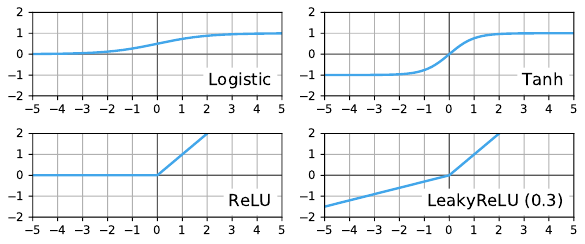
\includegraphics[width=12cm]{./statics/activation_functions.png}
    \caption{نمودار توابع فعال‌سازی معرفی شده}
\end{figure}

به عنوان تابع فعال‌سازی لایه آخر توصیه می‌شود از تابعی استفاده شود که بردی برابر
با بازه برچسب‌های \gls{dataset} داشته باشد. برای مثال اگر خروجی از جنس احتمال
است، تابع فعال‌سازی سیگموید که بردی آن بین صفر و یک است انتخاب مناسبی است. اگر
مسئله \gls{classification} با چند دسته است، تابع softmax توصیه می‌شود. این تابع
فعال سازی می‌تواند به ازای هر نرون خروجی، گرادیان مناسب را تولید کند. اگر مسئله
\gls{regression} است که خروجی محدودیتی ندارد استفاده از یک تابع فعال‌ساز خطی
توصیه می‌شود.

\subsection{تابع خطا}
آموزش در \gls{nn} با کمک تابع خطا رخ می‌دهد. با استفاده از تابع خطا می‌توانیم
توانایی شبکه در حل مسئله مورد نظر را ارزیابی کنیم. وقتی که مدل بتواند خروجی‌های
مناسب را به ازای ورودی‌های داده شده تولید کند، مقدار تابع خطا پایین خواهد بود.
هرچی که خروجی مدل از مقدار مورد نظر کمتر باشد، مقدار تابع خطا افزایش پیدا
می‌کند. پس در صورتی که ابزاری برای کاهش مقدار تابع خطا داشته باشیم می‌توان
جواب‌های درست به ازای ورودی‌های مختلف را به مدل آموزش دهیم. همچنین از مقدار تابع
خطا بر روی کل \gls{dataset} می‌توان استفاده کرد تا توانایی مدل‌های مختلف بر
مسئله مورد نظر را با هم مقایسه کنیم.

توابع خطا بسیار زیادی پیشنهاد شده‌اند که باید با توجه به ماهیت مسئله مورد هدف و
ساختار شبکه استفاده شده، تابع مناسب را از بین آن‌ها انتخاب کرد. به صورت کلی
توابع خطا را به دو دسته بزرگ می‌توان تقسیم کرد. توابع خطا مسائل
\gls{classification} و توابع خطا مسائل \gls{regression}. مسائل
\gls{classification} مسائلی هستند که در آن‌ها هدف اختصاص یک یا چند برچسب به
ورودی داده شده است. تابع Hinge و \gls{cross entropy} نمونه‌ای از توابع خطا مناسب
برای مسائل \gls{classification} هستند. مسائل \gls{regression} مسائلی هستند که در
آن‌ها هدف اختصاص یک یا چند مقدار عددی به ورودی داده شده است. \gls{mse} نمونه‌ای
از یک تابع خطا برای مسائل \gls{regression} است.

تابع \gls{cross entropy} محبوب‌ترین تابع خطا برای مسائل \gls{classification}
محسوب می‌شود. مقدار این تابع خطا بر اساس احتمال پیشبینی شده برای هر برچسب و
برچسب‌های صحیح هر نمونه محاسبه می‌شود و توسط رابطه زیر می‌توان آن را محسابه کرد:
\begin{equation}
    CrossEntropyLoss(y, y^\prime) = \sum_{c=1}^{M} y_i log(y_i^\prime)
\end{equation}
$M$ نشان دهنده تعداد برچسب‌های مختلف مسئله است که هر ورودی مطلق به یکی از آن‌ها
هست. $y_i$ نشان دهنده اختصاص برچسب $i$ به ورودی است. در صورتی که ورودی متعلق به
این گروه باشد، مقدار آن یک است. در غیر این صورت مقدار آن صفر است. همچنین
$y_i^\prime$ احتمال محاسبه توسط مدل برای برچسب $i$ است. معمولا از softmax به
عنوان تابع فعال سازی همراه این تابع خطا استفاده می‌شود.

در صورتی که تنها دو بر چسب مثبت و منفی داشته باشیم و بخواهیم احتمال یک خصوصیت در
ورودی را پیشبینی کنیم، از رابطه ساده شده زیر می‌توان استفاده کرد:
\begin{equation}
    BinaryCrossEntropyLoss(y, y^\prime) = -(y log(y^\prime)) + (1 - y)log(1 - y^\prime)
\end{equation}
sigmoid تابع فعال‌سازی است توصیه شده برای این تابع خطا است.

\gls{mse} یکی از توابع خطای محبوب برای مسائل \gls{regression} محسوب می‌شود. این
تابع خطا فاصله اقلیدوسی بین نقطه پیشبینی شده توسط شبکه و نقطه مورد هدف را محاسبه
می‌کند در نتیجه هرچی خروجی شبکه نامناسب‌تر باشد، مقدار تابع خطا بیشتر می‌شود.
مقدار خطا توسط رابطه زیر قابل مقایسه است:
\begin{equation}
    MSE(y, y^\prime) = \frac{1}{M} \sum_{c=1}^{M} (y_i - y_i^\prime)^2
\end{equation}
که $M$ اندازه ابعاد فضای خروجی است و $y^\prime$ نقطه پیشبینی شده توسط شبکه است.
همچنین $y$ نقطه هدف مورد نظر است.

\subsection{الگوریتم پس‌انتشار خطا}
\gls{backpropagation} یک روش برای محاسبه گرادیان تابع خطا نسبت به وزن‌های
سیناپس‌ها در شبکه‌های عصبی مصنوعی است. این روش معمولا به همراه یک الگوریتم
بهینه‌سازی، مانند \gls{gd}، به عنوان الگوریتم آموزش شبکه‌های عصبی مصنوعی به کار
گرفته می‌شود. هرچند معمولا به کل الگوریتم آموزش استفاده شده پس انتشار خطا گفته
می‌شود ولی در عمل، پس انتشار خطا تقریبا همان قاعده زنجیره‌ای مشتق است و تنها
وظیفه محاسبه گرادیان را بر عهده دارد.

الگوریتم بهینه سازی معمولا شامل دو گام است که متوالیا و به صورت پی‌در‌پی تکرار
می‌شوند: محاسبه گرادیان و بروزرسانی وزن‌ها. وقتی که یک بردار ورودی به شبکه داده
می‌شود، سیگنال‌های خروجی لایه‌ها به ترتیب محاسبه می‌شود تا خروجی آخرین لایه شبکه
به دست آید. به این مرحله \gls{feedforward} گفته می‌شود. سپس مقدار لایه آخر با
مقدار دلخواه ما مقایسه می‌شود و با توجه به اختلاف آن‌ها یک مقدار خطا محاسبه
می‌شود. سپس از این خطا نسبت به وزن‌های لایه آخر گرادیان گرفته می‌شود و این مقدار
گرادیان با توجه به قاعده زنجره‌ای مشتق به لایه‌های قبل منتقل می‌شود و سهم هر
سیناپس در مقدار خطا محاسبه می‌شود. این مرحله \gls{backpropagation} نام دارد. در
نهایت گرادیان محاسبه شده به الگوریتم بهینه‌سازی داده می‌شود تا وزن جدید هر
سیناپس محاسبه شود.

در طی فرآیند آموزش هر نرون یاد می‌گیرد طوری وزن‌های خود را تغییر دهد که نرون‌های
مختلف نشان دهنده خصوصیت‌های مختلفی از ورودی شبکه‌ باشد. وقتی که آموزش شبکه به
پایان رسید، وقتی ورودی که حاوی الگویی است که یک نرون شبکه به آن حساس شده است، به
شبکه داده می‌شود، آن نرون از خود فعالیت بیشتری نشان می‌دهد.

همان گونه که گفته شد برای محاسبه مقدار خطا در این روش نیاز به دانستن خروجی مطلوب
شبکه در مرحله آموزش است. به این جهت روش آموزش \gls{backpropagation}، معمولا یک
روش \gls{supervised learning} محسوب می‌شود هر چند در معماری‌هایی همچون
\gls{autoencoder}، از این الگوریتم برای آموزش بدون نظارت استفاده می‌شود.

هرچند که در تئوری لازمه این روش این است که توابع فعال‌ساز استفاده شده در شبکه
توابعی مشتق‌پذیر باشند، ولی در عمل توابعی همچون ReLU که در یک یا چند نقطه از
دامنه خود مشتق پذیر نیستند هم می‌توان استفاده کرد.

\subsection{الگوریتم‌های بهینه‌سازی}
آموزش شبکه‌های عصبی در اصل یک فرایند بهینه‌سازی است که طی آن تلاش می شود وزن‌های
شبکه به گونه‌ای تنظیم شوند که مقدار تابع خطا کمینه شود. در عمل \gls{sgd}
الگوریتم پایه‌ای است که برای آموزش شبکه‌های عصبی از آن استفاده می‌شود. این
الگوریتم به صورت پی‌درپی وزن‌های شبکه را با توجه به یک نمونه از \gls{dataset} به
گونه‌ای تغییر می‌دهد که مقدار تابع خطا کاهش پیدا کند. همچنین بار محاسباتی
\gls{sgd} در مقایسه با \gls{gd} که کل \gls{dataset} را در هر مرحله در نظر
می‌گرد به شدت کمتر است.

در طی فرآیند یادگیری میزان تاثیر هر مرحله توسط نرخ یادگیری کنترل می شود. نرخ
یادگیری پایین‌تر باعث می‌شود که درنهایت شبکه به نقطه‌ای بهینه‌تر همگرا شود در
حالی که زمان آموزش را به شدت افزایش می‌دهد. نرخ یادگیری بالاتر باعث می‌شود که
سرعت کاهش خطا بیشتر شود ولی ممکن است فرآیند یادگیری را بی‌ثبات کند و مانع همگرا
شدن شبکه شود. برای کنترل نوسانات \gls{SGD} پیشنهاد شد که از مفهوم \gls{momentum}
استفاده شود. \gls{momentum} که از قانون اول نیوتون الهام گرفته است، باعث همگرایی
سریع‌تر شبکه می‌شود و همچنین دقت نهایی در مقایسه با \gls{sgd} ساده افزایش می‌دهد.

ایده اصلی \gls{momentum} این است که بجای این که تنها از گرادیان تابع خطا در همان
مرحله برای بروزرسانی وزن‌های شبکه استفاده شود، از میانگین گرادیان‌ها در مراحل
اخیر استفاده شود. این رفتار را می‌توان توسط روابط زیر مدل کرد:
\begin{equation}
    v := \gamma v - \eta \nabla J(w)
\end{equation}
\begin{equation}
    w := w + v
\end{equation}
که $v$ مقدار \gls{momentum} را مشخص می‌کند. همچنین $\gamma$ ضریب تاثیر
\gls{momentum} است که مقداری بین صفر و یک دارد. یکی از مزایای مهم استفاده از
\gls{momentum} در آموزش شبکه این است که از گیر کردن شبکه در نقاط کمینه محلی
جلوگیری می‌کند. مقدار بالا $\gamma$ می‌تواند باعث شود که آموزش شبکه بی‌ثبات شود
و از نقاط کمینه دور شود. معمولا این مقدار برابر نیم قرار داده می‌شود و بعد از
گذشت مدتی از آموزش، مقدار آن افزایش داده می‌شود.

همچنین برای تنظیم مقدار صحیح نرخ یادگیری روش‌های متفاوتی پیشنهاد شده است. یکی از
این روش‌ها این است که مقدار نرخ یادگیری به صورت پویا در طول آموزش کاهش پیدا کند
تا شبکه در ابتدا سریع‌تر و در ادامه با دقت بالاتری آموزش داده شود. همچنین مقدار
دادن به نرخ یادگیری با توجه اندازه گرادیان‌ها در مراحل قبل نیز می‌تواند به
پایداری فرآیند آموزش کمک بسیاری بکند. نام این روش نرخ یادگیری انطباقی است.

Adagrad اولین الگوریتم بهینه‌سازی بود که توانست با موفقیت از نرخ یادگیری
انطباقی برای آموزش شبکه‌های استفاده کند. این الگوریتم با استفاده از نگهداری
مجموع مربعات گردایان مراحل قبل هر سیناپس، مقدار نرخ یادگیری را برای پارامترهایی
که کمتر تغییر می‌کند زیاد می‌کند و با کاهش نرخ یادگیری مانع تغییر پارامترهایی
می‌شود که تغییرات زیادی دارند. با توجه به این که مجموع مربعات گردایان‌ها همیشه
مقداری مثبت و افزایشی هست، نرخ یادگیری پس از مدتی به صفر نزدیک می‌شود و آموزش
شبکه متوقف می‌شود.

برای حل این معضل، الگوریتم Adadelta معرفی شد. این الگوریتم با معرفی یک پارامتر
$\beta_2$ میزان تاثییر گرادیان‌های گذشته را مشخص می‌کند و جلوی کم شدن بیش از حد
نرخ یادگیری را می‌گیرد. این الگوریتم از محاسبه مجموعه مربعات گرادیان‌ها از رابطه
زیر استفاده می‌کند:
\begin{equation}
    E[g^2]_t = \beta_2 E[g^2]_{t-1} + (1 - \beta_2)g_t^2
\end{equation}
که $E[g^2]_t$ مجموع مربعات گرادیان‌ها در مرحله $t$ است. همچنین $g_t^2$ مربعات
گردیان‌ها در مرحله $t$ است.

در زمان نوشتن این پایان‌نامه، Adam محبوب‌ترین الگوریتم بهینه‌سازی برای شبکه‌های
عصبی است \cite{kingma2014adam}. همچنین در عمل نشان داده شد است که اکثر شبکه‌هایی
که با این الگوریتم، به‌جای سایر الگوریتم‌های بهینه‌سازی، آموزش داده می‌شوند از
دقت بهتری بهره‌مند هستند.

Adam نیز از نرخ یادگیری انطباقی برای آموزش شبکه استفاده می‌کند. ولی بر خلاف
الگوریتم‌هایی که در بالا توضیح داده شد، نه تنها از مربع گرادیان‌های قبلی، بلکه
از مقدار گرادیان‌های مراحل قبل نیز برای محاسبه نرخ یادگیری بهره می‌برد. استفاده
از گردیان مرحله‌های قبلی بسیار شبیه الگوریتم‌های برپایه \gls{momentum} است. با
این تفاوت از نظر فیزیکی \gls{momentum} رفتاری شبیه به یک توپ دارد که در سراشیبی
در حرکت است. ولی Adam رفتاری مانند یک توپ سنگین با اصطحکاک دارد. در نتیجه این
الگوریتم سطوح صاف در فضای بهینه‌سازی را ترجیح می‌دهد. این رفتار منجر به توانای
بالاتر شبکه‌های آموزش دیده شده با Adam می‌شود.

تاثیر گرادیان‌ها و مربعات گرادیان‌های مراحل قبل به کمک $m_t$ و $v_t$ انجام
می‌شود که توسط روابط زیر قابل محاسبه هستند:
\begin{equation}
    m_t = \beta_1 m_{t-1} + (1 - \beta_1) g_t
\end{equation}
\begin{equation}
    v_t = \beta_2 v_{t-1} + (1 - \beta_2) g_t^2
\end{equation}
همچنین از صفر برای مقدار اولیه این متغیرها استفاده می‌شود. همچنین مشاهده شد که
این متغیرها در مراحل اولیه آموزش به صفر متمایل هستند که باعث کاهش سرعت آموزش
می‌شود. از این جهت از روی این متغیرها دو متغیر دیگر $\hat{m_t}$ و $\hat{v_t}$ با
کمک روابط زیر محاسبه می‌شود:
\begin{equation}
    \hat{m_t} = \frac{m_t}{1 - \beta_1}
\end{equation}
\begin{equation}
    \hat{v_t} = \frac{v_t}{1 - \beta_2}
\end{equation}

با محاسبه مقادیر بالا می‌توان از رابطه زیر استفاده کرد تا وزن‌های شبکه در زمان
$t$، $w_t$، را محاسبه کرد:
\begin{equation}
    w_{t+1} = w_{t} - \frac{\eta}{\sqrt{\hat{v_t}} + \epsilon} \hat{m_t}
\end{equation}

همچنین طی بررسی‌های انجام شده برای $\beta1$ مقدار ۰/۹، برای $\beta2$ مقدار ۰/۹۹۹
و برای $\epsilon$ مقدار $10^{-8}$ پیشنهاد شد.

\subsection{مشکلات شبکه‌های عصبی عمیق}
آموزش شبکه‌های عصبی مشکلات مختلفی دارد ولی دوتا از رایج‌ترین مشکلات \gls{overfit} و
زمان‌بر بودن آموزش آن‌ها است.

شبکه‌های عصبی عمیق به علت پارامترها و لایه‌های زیاد می‌توانند جزئی‌ترین اطلاعات
موجود در داده آموزشی را هم مدل کنند. این خاصیت باعث می‌شود که این شبکه‌ها به
سرعت بیش برازش شوند و خاصیت تعمیم‌دهی خود را از دست بدهند. برای همین از روش‌های
مختلفی برای مقابله با این پدیده در این شبکه‌ها استفاده می‌شود.

یکی از بدیهی‌ترین و کاراترین این روش‌ها افزایش داده‌های آموزشی است. هرچه
داده‌های آموزشی بیشتر و متنوع‌تر باشند شبکه در مقابل \gls{overfit} مقاوم‌تر می‌شود و
بهتر می‌تواند برای ورودی‌های جدید تصمیم مناسب را بگیرد. ولی این روش علی رغم
کارایی بالا به علت هزینه زیادی به همراه دارد نمی‌توان در همه موارد از آن استفاده
کرد.

یک راه دیگر برای مقابله با \gls{overfit} استفاده از روش‌های \gls{regularization}
است. این روش‌ها از طریق اضافه کردن جملاتی به تابع خطا، مانند مجموع مربع وزن
سیناپس‌ها، بر روی آزادی شبکه محدودیت‌ها قرار می‌دهند که باعث می‌شود شبکه از تمام
توان خود استفاده نکند و فقط از توان مورد نیاز بهره ببرد. \gls{regularization} را
می‌توان در روی اجزای مختلفی از شبکه اعمال کرد ولی وزن‌های سیناپسی و فعالیت
نرون‌ها دو مورد از رایج‌ترین موارد برای منظم‌سازی اند.

علاوه بر منظم‌سازی، dropout یک روش دیگر برای کنترل توان شبکه است. به این صورت که
در مرحله آموزش شبکه، در هرلایه، به صورت تصادفی، تعداد از نرون‌ها پوشیده می‌شوند
و خروجی آن‌ها به لایه بعد منتقل نمی‌شود. پس از پایان آموزش خروجی در نرون در
ضریبی ضرب می‌شود تا توزیع احتمالی سیگنال ورودی به هر لایه و نرون برابر مرحله
آموزش بماند. به این ترتیب شبکه‌ هر خصوصیت را به چند صورت یاد می‌گیرد و مانع
\gls{overfit} می‌شود.

شبکه‌های عصبی عمیق \gls{hyper parameter} بسیاری همچون تعداد و اندازه لایه‌ها،
مقدار اولیه وزن‌ها، نرخ یادگیری، ضرایب منظم‌سازی و ضریب dropout دارند. از طرفی
در هر بار آموزش یک شبکه عصبی عمیق، میلیون‌ها پارامتر باید یادگرفته شوند که مدت
زمان هر آموزش را بسیار طولانی می‌کند. برای همین امتحان تمامی مقادیر برای پیدا
کردن بهترین ساختار ممکن است به علت محدودیت زمانی ممکن نباشد. ولی با این حال
روش‌هایی مانند \gls{batching} برای کاهش زمان یادگیری وجود دارند. به این صورت که
بجای نمایش یک مثال در هر مرحله، مجموعه‌ای از مثال‌‌ها به شبکه نشان داده می‌شود و
وزن‌ها به اندازه میانگین تغییر وزن هر مثال، تغییر داده می‌شوند. دسته‌بندی باعث
کاهش زمان آموزش و افزایش عملکرد شبکه می‌شود.

همچنین استفاده از \gls{GPU} ها، به علت این که می‌توان در آن‌ها هزاران محاسبه همزمان
انجام داد، به شدت برای آموزش شبکه‌های عصبی عمیق مناسب است و زمان آموزش آن‌ها را
کاهش می‌دهد.

علاوه بر مشکلات اشاره شده، آموزش شبکه‌های عصبی عمیق از مشکلاتی دیگری همچنون محو
شدن گرادیان‌ هم رنج می‌برد که با استفاده از تابع‌های فعال‌سازی همچون ReLU و یا
استفاده از ساختارهایی همچون \gls{batch normalization} می‌توان با آن مقابله کرد.
\chapter{آزمایش‌ها انجام شده}
\section{مجموعه داده}
با توجه به این که \gls{atm} یک مسئله \gls{supervised learning} محسوب می‌شود،
نیاز به \gls{dataset} است که برچسب گذاری شده باشد. به صورت کلی \glspl{dataset}
مورد استفاده در این مسئله مجموعه‌ای از زوج مرتب‌های فایل صوتی ضبط شده از یک قطعه
و همچنین آوانویسی آن قطعه می‌شود. این آوانویسی‌ها عموما به شکل فایل‌های
\gls{MIDI} هستند که در آن‌ها فعال و غیرفعال شدن نت‌ها به شکل دنباله‌ای از
رخدادها مشخص شده است. هر رخداد علاوه بر اطلاعات خود رویداد مشخص می‌کند که با چه
فاصله‌ی زمانی از آخرین رخداد قرار دارد. برای سازی مانند پیانو علاوه بر اطلاعات
فعال و غیرفعال شدن نت‌ها، رخدادهایی نیز برای مشخص کردن فعال و غیرفعال شدن
پدال‌ها در نظر گرفته شده است.

\subsection{MAPS}
MAPS یک \gls{dataset} از فایل‌های \gls{MIDI} و فایل‌های صوتی هم‌تراز آن‌ها است
که برای مسائل \gls{atm} و \gls{mpe} طراحی و آماده‌سازی شده است
\cite{emiya2009multipitch}. فایل‌های صوتی در شرایط محیطی مختلف ضبط شده‌اند و از
استاندارد CD تبعیت می‌کنند. به این معنی که هر نمونه ۱۶ بیت دقت دارد و نمونه
برداری با دقت ۴۴ کیلوهرتز انجام شده است. این \gls{dataset} شامل حدود ۶۵ ساعت
فایل صوتی است و حجم کل \gls{dataset} در حدود ۴۰ گیگابایت است. MAPS تحت مجوز
\rl{Creative Commons} به صورت عمومی منتشر شده است.

برای تولید MAPS ابتدا مجموعه‌ای عظیم از فایل‌ها \gls{MIDI} جمع‌آوری شده است. سپس
از فایل‌های \gls{MIDI} جمع‌آوری شده استفاده شده تا فایل صوتی متناظر هر کدام
تولید شود. برای تولید فایل‌های صوتی کاملا هم‌تراز با فایل‌های \gls{MIDI} از دو
روش استفاده شده است.

عمده فایل‌ها توسط نرم‌افزار ایجاد شده‌اند و از هیچ ساز فیزیکی برای تولید آن‌ها
استفاده نشده است. برای این مجموعه از فایل‌ها ابتدا فایل‌های \gls{MIDI} پشت هم
قرار داده شده‌اند تا فایل‌های \gls{MIDI} کمتر ولی با طولی بیشتر به دست آید. سپس
خروجی صوتی هر فایل توسط نرم‌افزار \lr{Steinberg’s Cubase SX} شبیه‌سازی شده است.
برای ایجاد تنوع در فایل‌های صوتی، نرم‌افزار جهت انجام شبیه‌سازی برای فایل‌های
مختلف از نمونه اجراهای پیانوهای مختلف و در شرایط محیطی متفاوت استفاده کرده است.
در نهایت فایل‌های صوتی ایجاد شده با توجه به فایل‌های \gls{MIDI} ابتدایی قطعه
قطعه شده‌اند تا اجرای متناظر هر فایل به دست آید. دلیل استفاده از فایل‌های
طولانی‌تر بجای استفاده از فایل‌های اصلی این بوده است که نرم‌افزار استفاده شده به
صورت اتوماتیک قابل کنترل نیست و برای هر ایجاد هر فایل نیز به دخالت انسانی است.

برای بخش دیگر از فایل‌های صوتی از یک پیانو Disklavier استفاده شده است. این
خانواده از پیانوها می‌توانند از طریق ارتباط \gls{MIDI} فشرده شدن هر کلاویه را با
قدرت‌های مختلف شبیه‌سازی کنند. در نتیجه مانند این است که یک نوازنده با قدرتی
فراانسانی هر کلاویه را در زمان درست و با \gls{velocity} مشخص شده فشار دهد و
دقیقا در زمان خواسته شده آن‌را رها کند. همچنین برای ایجاد تنوع در فایل‌های صوتی
ضبط شده در گروهی از فایل‌ها میکروفن در فاصله نیم‌متری ساز قرار داده شده است و در
گروه دیگر میکروفن در فاصله‌ای مابین ۳ تا ۴ متری ساز قرار دارد.

نکته قابل توجه این است که فایل‌های \gls{MIDI} که برای تولید صوت در روش‌های مختلف
استفاده شده است ممکن است اشتراک داشته باشند. در نتیجه از یک قطعه ممکن است چندین
اجرای مختلف موجود باشد.

در این \gls{dataset} چهار دسته فایل \gls{MIDI} و اجراهای متناظر آن‌ها وجود دارد:
\begin{enumerate}
    \item فقط شامل اجرای مجرد نت‌های مختلف و اجراهای کوتاه
    \gls{monophonic} است. از این بخش از \gls{dataset} می‌تواند برای روش‌هایی
    مانند \gls{nmf} که نیاز به اجرای جدای نت‌ها دارند استفاده کرد.

    \item  شامل اجرای \glspl{chord} می‌شود که نت‌ها با هم هیچ ارتباط
    موسیقیایی ندارند و به صورت تصادفی در کنار هم قرار گرفته‌اند. این بخش از
    \gls{dataset} برای آزمایش عملکرد مدل‌های \gls{mpe} بدون استفاده‌ای از دانش
    موسیقی مناسب است.

    \item شامل اجرا \glspl{chord} رایج در موسیقی‌های غربی، مانند \glspl{chord}
    جز و یا \glspl{chord} کلاسیک، است. در نتیجه این بخش از \gls{dataset} برای
    سیستم‌هایی که از دانش موسیقیایی برای افزایش  دقت استفاده می‌کنند مناسب است.

    \item شامل ۲۳۸ قطعه موسیقی کلاسیک هست که در زمان انتشار \gls{dataset} تحت
    مجوز \rl{Creative Commons} منتشر شده بودند. تمام این فایل‌ها به صورت دستی
    پردازش شده‌اند تا هر نت کشش و \gls{velocity} مناسب را داشته باشد. این بخش از
    \gls{dataset} برای سیستم‌های \gls{atm} مناسب است.
\end{enumerate}

در این پایان‌نامه فقط از فایل‌های صوتی ضبط شده از اجرای Disklavier برای ارزیابی
استفاده شده است. دلیل این انتخاب این است که در دنیای واقعی هدف آوانویسی اجراهای
یک ساز واقعی است و اجراهای مصنوعی که توسط نرم‌افزار تولید شده‌اند اکثر جزییات یک
ساز واقعی را ندارند. همچنین تنها قطعات کامل مورد استفاده قرار گرفته‌اند تا مجددا
ارزیابی واقعاگرایانه‌تری انجام شود. در نهایت قطعات انتخاب شده دقیقا همان قطعات
استفاده شده برای ارزیابی در مدل‌های پیشنهاد شده پیشین است
\cite{hawthorne2017onsets,hawthorne2018enabling}.

علارغم تمام تلاش‌های انجام شده در تهیه این \gls{dataset} همچنان چندین مشکل وجود
دارد. مشکل اول حجم کم داده است. برای مثال این \gls{dataset} تنها شامل ۶۰ نمونه
از اجرای ضبط شده واقعی است که با توجه به ماهیت مسئله بسیار محدود است. همچنین بجز
حجم کم داده، در چندین مورد فایل‌های \gls{MIDI} با نسخه‌های ضبط شده هم‌خوانی کامل
ندارند. برای مثال در قطعات مختلف اجرا نشدن نت‌های با \gls{velocity} پایین کاملا
محسوس است.

\subsection{MAESTRO}
MAESTRO یک \gls{dataset} است که توسط \cite{hawthorne2018enabling} برای رفع
مشکلات MAPS معرفی شد. این \gls{dataset} شامل بیش از ۱۷۰ ساعت اجرای موسیقی است که
طی ۱۰ سال در مسابقات \lr{Piano-e-Competition} جمع‌آوری شده است.

تمام این قطعات در کیفیت CD یا بالاتر هستند. همچنین در آوانویسی اطلاعات
\gls{velocity} نت‌ها و تغیرات پدال نگه‌دارنده نیز لحاظ شده است. آوانویسی و
اجراها با دقت ۳ میلی‌ثانیه تراز شده‌اند که حاکی از کیفیت بسیار بالای این
\gls{dataset} است. همچنین علاوه بر آوانویسی برای هر قطعه اطلاعات اضافه‌ دیگری
مانند آهنگ‌ساز و سال اجرا نیز موجود است. عمده قطعات این \gls{dataset} قطعات
کلاسیک ما بین قرن هفدهم و بیستم هستند.

این \gls{dataset} به صورت پیش‌فرض به سه بخش آموزش، صحت‌سنجی و ارزیابی به گونه‌ای
تقسیم شده است که اجراهای متفاوت از یک قطعه در بخش‌ها متفاوت قرار نگیرند. در جدول
زیر اطلاعات مربوط به هر بخش نشان داده شده است.
\begin{table}[ht]
    \centering
    \begin{tabular}{|c|c|c|c|c|c|}
        \hline
        بخش & تعداد اجرا & تعداد قطعه & زمان به ساعت & حجم به گیگابایت & تعداد نت به میلیون \\
        \hline
        آموزش & ۹۵۴ & ۲۹۵ & ۱۴۰/۱ & ۸۳/۶ & ۵/۰۶ \\
        \hline
        صحت‌سنجی & ۱۰۵ & ۶۰ & ۱۵/۳ & ۹/۱ & ۰/۵۴ \\
        \hline
        ارزیابی & ۱۲۵ & ۷۵ & ۱۶/۹ & ۱۰/۱ & ۰/۵۷ \\
        \hline
        مجموع & ۱۱۸۴ & ۴۳۰ & ۱۷۲/۳ & ۱۰۲/۸ & ۶/۱۸ \\
        \hline
    \end{tabular}
    \caption{اطلاعات \gls{dataset} MAESTRO}
\end{table}

\section{معیارهای ارزیابی}
معیارهای استفاده شده برای ارزیابی بسیار نزدیک به معیارهای پیشنهاد شده در مسابقات
MIREX است که توسط کتابخانه \lr{mir-eval} \cite{raffel2014mir_eval} پیاده‌سازی
شده‌اند.

برای ارزیابی ابتدا از \gls{dataset} مجموعه‌ای از سه‌تایی‌های مرتب مرتبط با هر
قطعه استخراج می‌شود. هر کدام از این سه‌تایی‌های مرتب نشان دهنده یک نت هستند و
اعضای آن به ترتیب فرکانس نت، زمان شروع و زمان پایان نت را نشان می‌دهند. به این
ساختار ذخیره‌سازی موسیقی دنباله نت می‌گوییم. همچنین پس از انجام آوانویسی توسط
مدل، خروجی مدل از ساختار \gls{pianoroll} توسط الگوریتمی که در ادامه بحث می‌شود
به دنباله نت تبدیل می‌شود.

برای ارزیابی نیاز هست که تشخیص دهیم که کدام یک از نت‌های تشخیص داده شده توسط مدل
واقعا در قطعه حضور دارند، چه تعداد حضور ندارند و مدل چه تعداد از نت‌ها را تشخیص
نداده است. همچنین با توجه به این که میزان کمی خطا در زمان‌ها و یا فرکانس نت‌های
تشخیص داده شده طبیعی است، معیارهای استفاده شده نیاز به مقداری انعطاف‌پذیری نیز
دارند.

به این منظور گرافی دو بخشی ایجاد می‌شود که راس‌های یک بخش نت‌های استراخ شده از
\gls{dataset} هستند و راس‌های بخش دیگر نت‌های تشخیص داده شده توسط مدل هستند. در
صورتی که بتوان دو راس مختلف از دو بخش را برابر دانست بین‌ آن‌ها یالی قرار
می‌دهیم در غیر این صورت دو راس به هم مرتبط نیستند. همچنین شرط برابر بودن نت‌ها
وابسطه به معیار متفاوت است که در ادامه برای هر معیار این شرط بررسی می‌شود.

پس از تشکیل گراف ذکر شده، تطابق بیشینه گراف محاسبه می‌شود تا مشخص شود که چه
نت‌هایی به درستی تشخیص داده شده‌اند و چه نت‌های اشتباه تشخیص داده شده‌اند و یا
تشخیص داده نشده‌اند. پس از محاسبه این تطابق می‌توان از طریق روابط زیر مقادیر
\gls{precision}، \gls{recall} و F1 را برای معیار مورد نظر محاسبه کرد:
\begin{equation}
    precision = \frac{TP}{TP + FP}
\end{equation}
\begin{equation}
    recall = \frac{TP}{TP + FN}
\end{equation}
\begin{equation}
    F1 = 2 \frac{precision . recall}{precision + recall}
\end{equation}

$TP$ تعداد نت‌هایی هست که به درستی تشخیص داده شده‌اند که برابر با اندازه تطابق
محاسبه شده است. $FP$ نت‌هایی هستند که مدل تشخیص داده است ولی واقعا وجود ندارند.
این عدد برابر با راس‌های از بخش مربوط به نت‌های تشخیص داده شده توسط مدل هستند که
در تطابق نیستند. همچنین $FN$ تعداد نت‌هایی هست که مدل نتوانسته تشخیص دهد. تعداد
این نت‌ها برابر با راس‌هایی از بخش استخراج شده از \gls{dataset} است که عضو تطابق
نیستند.

شرط برابر فرض شدن دو نت با توجه به معیار مورد نظر متفاوت است. معیار اول فقط به
شروع نت‌ها تشخیص داده شده اهمیت می‌دهد. در نتیجه دو نت یکسان فرض می‌شوند اگر
\gls{pitch} آن‌ها کمتر از ربع‌پرده اختلاف داشته باشد و همچنین تفاوت زمان شروع
آن‌ها کمتر از ۵۰ میلی‌ثانیه باشد.

معیار بعدی علاوه بر شروع نت‌ها به زمان پایان نت‌ها نیز اهمیت می‌دهد. در نتیجه
برای برابر فرض شدن دو نت علاوه بر شروط قبلی، دو نت باید اختلاف زمان پایانشان
کمتر از بیشینه ۵۰ میلی‌ثانیه و یک پنچم طول نت مرجع باشد.

\section{تبدیل دادگان}
اطلاعات موجود در \gls{dataset} به صورت مستقیم برای آموزش مدل و ارزیابی عملکرد آن
قابل استفاده نیستند. فایل‌های صوتی ابتدا نیاز دارند تا به نرخ نمونه‌گیری شانزده
کیلوهرتز برده شوند و سپس سیگنال به دست آمده تبدیل به \gls{spec} شود. همچنین
فایل‌های \gls{MIDI} باید تبدیل به نمایش دنباله نت شوند. در فاز آموزش این
دنباله نت‌های به دست آماده تبدیل به \gls{pianoroll} می‌شوند تا برچسب‌ها مورد
نیاز آموزش شبکه به دست آید. همچنین با توجه به این که خروجه شبکه نیز یک
\gls{pianoroll} است، برای ارزیابی به فرآیندی برای تبدیل مجدد به دنباله نت نیاز
است. در ادامه هر کدام از این تبدیل‌ها بررسی می‌شوند.

\subsection{تبدیل صوت به اسپکتروگرام}
در قدم اول نیاز هست تا فایل‌های صوتی \gls{dataset} به نرخ نمونه‌گیری شانزده
کیلوهرتز برده شوند. با توجه به این که زیرترین نت پیانو فرکانسی برابر ۴۱۸۶ هرتز
دارد، پس نرخ نمونه‌گیری شانزده کیلوهرتز می‌تواند تمام اطلاعات نت‌ها را نگه‌دارد
و بخش ارزشمندی از اطلاعات از دست نرود. همچنین در صورتی که صوتی ورودی بیشتر از یک
کانال داشته باشد قبل از تغییر نرخ نمونه‌گیری، با میانگین گرفتن بین کانال‌های
مختلف، صوت را تبدیل به یک سیگنال تک‌کاناله می‌کنیم.

در قدم بعدی نیاز است که این سیگنال صوتی به دست آمده به فضای فرکانس برده شود.
برای این منظور بر روی سیگنال به دست آماده تبدیل mel را اعمال می‌کنیم. در این
تبدیل از پنجره هان به طول ۲۰۴۸ نمونه، برابر ۱۲۸ میلی‌ثانیه، برای محاسبه فرم‌ها
استفاده می‌شود. همچنین در هر مرحله پنجره را اندازه ۵۱۲ نمونه، برابر ۳۲
میلی‌ثانیه، حرکت می‌دهیم. بم‌ترین فرکانس محاسبه شده برابر ۳۰ هرتز است و در نهایت
\gls{spec} خروجی به ازای هر فرم، یک بردار با اندازه ۲۲۹ خواهد بود.

\subsection{تبدیل MIDI به دنباله‌ی نت}
اطلاعات در فایل‌های \gls{MIDI} به شکل دنباله‌ای از رخدادها ذخیره می‌شوند. هر
رخداد از سه بایت تشکیل شده که شامل اطلاعاتی همچنین نوع رخداد و فاصله زمانی از
رخداد قبلی می‌شود. مهم‌ترین این رخدادها رخدادهای فعال شدن و غیر فعال شدن نت‌ها
هستند. همچنین در پیانو رخداد تغییر وضعیت پدال \gls{sustain} نیز اهمیت زیادی
دارد.

پدال \gls{sustain} در پیانو به این شکل عمل می‌کند که در زمان فشرده بودن پدال حتی
اگر کلاویه توسط نوازنده رها شود، نت همچنان فعال می‌ماند. نت فعال تنها در صورت
تمام می‌شود نوازنده مجددا همان کلاویه را فشار دهد یا پدال \gls{sustain} را رها
کند. در نتیجه برای تولید دنباله‌ی نت از فایل \gls{MIDI} توجه به تغییرات پدال
\gls{sustain} لازم است در دنباله نت خروجی باید هر نت تا پایان فعال بودن پدال،
فعال نگه‌داشته شود.

\section{تبدیل دنباله‌ی نت به رول پیانو}
هر \gls{pianoroll} شامل دو ماتریس است که به ترتیب نشان‌دهنده فعال شدن و غیر فعال
شدن نت‌ها می‌باشند. هر ماتریس ۸۸ ستون دارد که متناظر با ۸۸ کلاویه پپانو است.
همچنین هر سطر از این ماتریس‌ها نماینده یک فرم است.

به صورت سنتی ماتریس دوم بجای نشان‌دهنده غیرفعال شدن یک نت، نشان‌دهنده فعال بودن
یا نبودن هر نت در یک فرم بوده است. با توجه به این موضوع که تشخیص غیرفعال شدن نت
در صوت، به علت ایجاد تفاوت محسوس‌تر بین دو فرم متوالی، ساده‌تر است، در این
پایان‌نامه تصمیم گرفته شد که بجای تشخیص فعال بودن نت‌ها، غیرفعال شدن هر نت تشخیص
داده شود.

برای تبدیل کافی است تا زمان شروع و پایان هر نت بر طول هر فرم، که در این
پایان‌نامه برابر ۳۲ میلی‌ثانیه است، تقسیم شود تا شماره ستون فرم متناظر به دست
آید. سپس در ماتریس اول درایه متناظر با کلاویه و فرم شروع فعال شدن نت و در ماتریس
دوم درایه متناظر با کلاویه و فرم غیر فعال شدن نت یک شود. همچنین اگر فرم فعال شدن
و غیر فعال شدن یک نت یکی شد، از آن نت صرف نظر می‌شود. شبه کد زیر الگوریتم تبدیل
دنباله نت به \gls{pianoroll} را نشان داده است.

\begin{algorithm}[ht]
\caption{تبدیل دنباله نت به \gls{pianoroll}}
\begin{algorithmic}
\begin{latin}
    \Require $notesequence$
    \Ensure $onsets$, $offsets$
    \State $notesequence\_duration \leftarrow$ max of all end times
    \State $num\_frames \leftarrow \lfloor notesequence\_duration / frame\_duration \rfloor + 1$
    \State $onsets \leftarrow$ zero matrix of size $num\_frames \times 88$
    \State $offsets \leftarrow$ zero matrix of size $num\_frames \times 88$
    \For {$note$ in $notesequence$}
        \State $pitch \leftarrow note.pitch$
        \State $onset \leftarrow \lfloor note.start\_time / 0.032 \rfloor$
        \State $offset \leftarrow \lfloor note.end\_time / 0.032 \rfloor$
        \If {$onset$ is $end$}
            \State continue
        \EndIf
        \State $onsets_{onset, pitch} \leftarrow 1$
        \State $offsets_{offset, pitch} \leftarrow 1$
    \EndFor
\end{latin}
\end{algorithmic}
\end{algorithm}

\subsection{تبدیل رول پیانو به دنباله‌ی نت}
برای ارزیابی عملکرد مدل لازم است تا \gls{pianoroll} تولید شده توسط مدل به یک
دنباله نت تبدیل شود. با این که به صورت سنتی از \gls{hmm} برای این تبدیل استفاده
می‌شود ولی نشان داده شده است که یک الگوریتم ساده نیز می‌تواند نتایج مشابه بدهد و
نیازی به سربار محاسباتی اضافه \gls{hmm} وجود ندارد.

کافی است که به ازای هر \gls{pitch}، در ستون متناظر با آن از ابتدا شروع به حرکت
کنیم. اگر در ماتریس اول مقدار یک درایه بیشتر از حدنساب ۰/۵ شد نت مورد بررسی از
آن فرم به بعد فعال فرض می‌شود. اگر به ازای یک نت فعال مجددا تشخیص فعال شدن نت
داده شد، نت فعال قبلی تمام می‌شود و نت دیگری از آن‌جا آغاز می‌شود. هرگاه در
ماتریس دوم مقدار پیش‌بینی شده از حدنساب بیشتر شد، در صورت موجود بودن یک نت فعال،
آن نت تمام شده فرض می‌شود. در شبه کد زیر الگوریتم تبدیل \gls{pianoroll} به
دنباله‌ی نت نشان داده شده است.
\begin{algorithm}[ht]
\caption{تبدیل \gls{pianoroll} به دنباله‌ی نت}
\begin{algorithmic}
\begin{latin}
    \Require $onsets$, $offsets$
    \Ensure $notesequence$
    \State $notesequence \leftarrow \emptyset$
    \State $num\_frames \leftarrow onsets.shape[0]$
    \For {$pitch$ from $0$ to $88$}
        \State $start \leftarrow null$
        \For {$frame$ from $0$ to $num\_frames$}
            \State $is\_onset \leftarrow onsets_{frame, pitch} \geq 0.5$
            \State $is\_offset \leftarrow offsets_{frame, pitch} \geq 0.5$
            \If {$is\_onset$ and $start$ is $null$}
                \State $start \leftarrow frame$
            \ElsIf {$is\_onset$ and $start$ is not $null$}
                \State $note \leftarrow Note()$
                \State $note.pitch \leftarrow pitch$
                \State $note.start\_time \leftarrow start * 0.032$
                \State $note.end\_time \leftarrow frame * 0.032$
                \State $notesequence \leftarrow notesequence \cup note$
                \State $start \leftarrow frame$
            \ElsIf {$is\_offset$ and $start$ is not $null$}
                \State $note \leftarrow Note()$
                \State $note.pitch \leftarrow pitch$
                \State $note.start\_time \leftarrow start * 0.032$
                \State $note.end\_time \leftarrow frame * 0.032$
                \State $notesequence \leftarrow notesequence \cup note$
                \State $start \leftarrow null$
            \EndIf
        \EndFor
        \If {$start$ is not $null$}
            \State $note \leftarrow Note()$
            \State $note.pitch \leftarrow pitch$
            \State $note.start\_time \leftarrow start * 0.032$
            \State $note.end\_time \leftarrow num\_frames * 0.032$
            \State $notesequence \leftarrow notesequence \cup note$
        \EndIf
    \EndFor
\end{latin}
\end{algorithmic}
\end{algorithm}

\subsection{کوتاه‌سازی دنباله‌ها}
به علت طولانی بودن \gls{spec} و \gls{pianoroll} هیچ کدام از مدل‌های بررسی شده در
ادامه امکان بررسی یک دنباله کامل را به علت محدودیت حافظه ندارند. برای حل این
مشکل در زمان آموزش، هر دنباله به دنباله‌های کوچیک‌تر به طول ۱۰۰۰، برابر ۳۲
ثانیه، شکسته می‌شوند. همچنین اگر دنباله‌ای پس از تجزیه طولی کمتر از ۱۵۰، ۴/۸
ثانیه، داشته باشد از فرایند آموزش حذف می‌شود.

در زمان ارزیابی نیز این تجزیه لازم است. هر دنباله ورودی به مدل ابتدا به
دنباله‌هایی به طول حداکثر ۱۰۰۰ شکسته می‌شوند. همچنین به هر دنباله ۱۰۰ عضو قبلی و
بعدی، در صورت وجود، افزوده می‌شود. این عضوهای ورودی صرفا برای دادن اطلاعات محیطی
بیشتر به مدل هستند و از خروجی مدل حذف می‌شود. پس از آن که مدل کل یک دنباله را
مشاهده کرد، دنباله‌ها خروجی با توجه به ترتیب اولیه به هم متصل می‌شوند و سپس مورد
ارزیابی قرار می‌گیرند.

\section{آزمایش‌ها}
\subsection{مدل آوایی ساده}
در آزمایش اول تنها یک مدل آوایی بسیار ساده بررسی شده است. این مدل تنها شامل ۳
لایه پیچشی تک بعدی است که روی هم قرار گرافته‌اند. سپس خروجی لایه آخر به دو شبکه
\gls{fully connected} داده می‌شود تا دو ماتریس \gls{pianoroll} را تولید کنند.

هر لایه پیچشی استفاده شده در مدل کرنلی با اندازه سه دارند و شامل ۵۱۲
\gls{feature map} می‌باشند. دلیل استفاده از لایه پیچشی این است که بررسی تغییرات
هر فرم زمانی با داشتن اطلاعات فرم‌های اطراف بسیار ساده‌تر هست. این لایه‌ها از
تابع فعال‌ساز ReLU استفاده می‌کنند.

دولایه \gls{fully connected} خروجی هر کدوم شامل ۸۸ نرون خروجی می‌شوند. این دو
لایه بر روی هر فرم به صورت مستقل اعمال می‌شوند و از تابع فعال‌ساز sigmoid
استفاده می‌کنند. در نتیجه هر درایه ماتریس‌های خروجی مانند یک دسته‌بندی دوگانه
است که مشخص می‌کند هر نت در چه فرمی شروع شده و در چه فرمی پایان یافته است.

نکته قابل توجه در مورد این مدل این است که شامل هیچ ساختاری برای پردازش دنباله‌ی
اطلاعات نیست و تصمیم‌گیری در مورد فعال یا غیرفعال شدن نت‌ها در هر فرم تنها
بر اساس فرم‌های ورودی همسایه رخ می‌دهد. در نتیجه این مدل تقریبا هیچ گونه
اطلاعاتی درباره ساختار موسیقی را نمی‌تواند فرابگیرد.

برای محاسبه خطای خروجی‌ها از تابع خطای \gls{cross entropy} استفاده شده است. با
توجه به نامتوازن بودن برچسب‌های خروجی، درایه‌هایی که مقدار حقیقی آن‌ها یک بوده
است، خطایشان ابتدا در ۵ ضرب شده است و سپس از مقدار خطای کل درایه‌های دو ماتریس
میانگین گرفته شده است تا خطای نهایی بدست آید.

در طول آموزش از الگوریتم بهینه‌سازی ADAM برای تنظیم وزن‌های شبکه استفاده شده
است. همچنین مقدار نرخ یادگیری طی ۴۰۰۰ مرحله اولیه آموزش افزایش یافته است و سپس
مجددا کاهش داده شد. با استفاده از تابع زیر می‌توان مقدار نرخ یادگیری در هر مرحله
را محاسبه کرد:
\begin{equation}
    lr(step) =
    \begin{cases}
        0.003 * \frac{step}{4000} &\quad step \leq 4000\\
        0.003 * \frac{1}{\sqrt{step - 4000}} &\quad step > 4000\\
    \end{cases}
\end{equation}

پس از آموزش شبکه برای ۱۰۰۰۰ مرحله با اندازه دسته ۱۶ به نتایج زیر دست یافته شد:
\begin{table}[ht]
    \centering
    \begin{tabular}{|c|c|c|c|c|c|c|}
        \hline
        & \multicolumn{3}{|c|}{تنها شروع نت} & \multicolumn{3}{|c|}{شروع و پایان نت} \\
        \hline
        دیتاست & \gls{precision} & \gls{recall} & F1 & \gls{precision} & \gls{recall} & F1 \\
        \hline
        MAPS & ۰/۶۳۴ & ۰/۶۴۲ & ۰/۶۳۸ & ۰/۴۳۰ & ۰/۴۳۸ & ۰/۴۳۴ \\
        \hline
        MAESTRO & ۰/۷۶۰ & ۰/۷۶۲ & ۰/۷۶۱ & ۰/۶۱۳ & ۰/۶۰۹ & ۰/۶۱۱ \\
        \hline
    \end{tabular}
    \caption{نتایج مدل آوایی ساده}
\end{table}

\subsection{مدل آوایی پیچیده}
در مدل آوایی پیچیده به مدل این قابلیت داده شده است که علاوه بر توانایی بررسی
همسایگی هر فرم برای تشخیص فعال و غیرفعال شدن نت‌ها، بتواند به فرم‌های دورتر هم
نگاه کند و از اطلاعات آن‌ها نیز برای تصمیم گیری استفاده کند. به این ترتیب مدل
می‌تواند قوانین موسیقیایی را نیز به صورت ضمنی فرا بگیرد و از آن‌ها برای افزایش
دقت خود استفاده کند.

در ابتدا مجددا ۳ لایه پیچشی تک بعدی وجود دارد که ساختاری دقیقا مشابه لایه‌های
استفاده شده در مدل آوایی ساده دارند. خروجی پس از اعمال \gls{positional encoding}
به بخش \gls{encoder} یک \gls{transformer} داده می‌شود. این بخش به مدل این قابلیت
را می‌دهد که محتوای فرم‌های دورتر را نیز بررسی کند و بر اساس آن‌ها تصمیم بگیرد.
بخش \gls{encoder} استفاده شده شامل ۸ لایه می‌شود. \gls{multi-head attention}
استفاده شده در داخل آن ابعادی برای ۵۱۲ دارد و شامل ۴ سر می‌شود. همچنین لایه
\gls{fully connected} بعد از هر \gls{multi-head attention} ۲۰۴۸ نرون خروجی دارد.

در نهایت خروجی به دو لایه \gls{fully connected} مجزا داده می‌شود تا دو ماتریس
\gls{pianoroll} را پیش‌بینی کنند. این لایه‌ها هم کاملا مشابه لایه‌های \gls{fully
connected} انتهایی مدل آوایی ساده می‌باشند.

تابع خطا و الگوریتم بهینه‌سازی کاملا مشابه مدل آوایی ساده هستند. این مدل پس از
آموزش دیدن به ازای ۲۰۰۰۰ مرحله با اندازه دسته ۱۶ توانست به نتایج زیر دست پیدا
کند.
\begin{table}[ht]
    \centering
    \begin{tabular}{|c|c|c|c|c|c|c|}
        \hline
        & \multicolumn{3}{|c|}{تنها شروع نت} & \multicolumn{3}{|c|}{شروع و پایان نت} \\
        \hline
        دیتاست & \gls{precision} & \gls{recall} & F1 & \gls{precision} & \gls{recall} & F1 \\
        \hline
        MAPS & ۰/۷۱۰ & ۰/۷۱۱ & ۰/۷۱۰ & ۰/۵۱۶ & ۰/۵۱۲ & ۰/۵۱۴ \\
        \hline
        MAESTRO & ۰/۸۴۲ & ۰/۸۳۷ & ۰/۸۴۰ & ۰/۶۹۶ & ۰/۶۹۰ & ۰/۶۹۳ \\
        \hline
    \end{tabular}
    \caption{نتایج مدل آوایی پیچیده}
\end{table}

همان گونه که از نتایج مشخص است، با این که تنها تفاوت این مدل با مدل قبل اضافه
کردن ساختاری برای استفاده از اطلاعات به دست آماده از فرم‌های دورتر است، دقت این
مدل به شکل قابل توجهی افزایش یافته است. در نتیجه می‌توان گفت که مدل به صورت ضمنی
دارد قواعد موسیقی را در این لایه‌ها فرا می‌گیرد و با کمک آن‌ها پیش‌بینی لایه‌های
اولیه را بهبود می‌دهد.

\subsection{بکارگیری مدل موسیقیایی پیشنهادی}
در \gls{asr} استفاده از یک مدل زبانی که فقط بر روی متن آموزش دیده شده است و درک
مناسبی از قواعد زبانی دارد، می‌تواند دقت مدل آوایی را به خوبی افزایش دهد و نتایج
رضایت‌بخشی به دست آورد. در \gls{asr} مدل زبانی با کمک الگریتم جست‌جوی beam در هر
مرحله خروجی مدل آوایی را اصلاح می‌کند. در \gls{atm} به علت مشکلاتی مانند طول
بسیار زیاد دنباله‌های ورودی استفاده از الگریتم جست‌وجوی beam ممکن نیست. در
ادامه ابتدا یک روش آموزش مدل موسیقیایی را معرفی می‌شود. سپس یک روش برای ترکیب
این مدل با یک مدل آوایی بررسی می‌شود.

\subsubsection{مدل موسیقیایی}
این مدل تنها بر روی آوانویسی در شکل \gls{pianoroll} آموزش داده می‌شود. در نتیجه
مدل دو ورودی می‌گیرد که دو ماتریس \gls{pianoroll} می‌باشند. این دو ماتریس به هم
در بعد \gls{pitch} متصل می‌شود و سپس به سه لایه \gls{fully connected} پشت هم
داده می‌شوند. در کدام از این لایه‌ها ۵۱۲ خروجی دارند.

سپس در زمان آموزش ۳۰ درصد فرم‌های به دست آمده به صورت تصادفی انتخاب می‌شوند و
مقدار آن‌ها صفر می‌شود در نتیجه اطلاعات مربوط به آن فرم‌ها کاملا از دست می‌رود.
ماتریس جدید پس از اعمال \gls{positional encoding} به بخش \gls{encoder} یک مدل
\gls{transformer} با ساختاری کاملا مشابه ساختار استفاده شده در مدل آوایی پیچیده
داده می‌شود. خروجی این ساختار مجددا به دو لایه \gls{fully connected} داده می‌شود
که هر کدوم مربوط به یک ماتریس \gls{pianoroll} می‌باشند. این دو لایه نهایی نیز
ساختاری کاملا مشابه با مدل آوایی پیچیده دارند.

برای آموزش مدل از تابع خطا و الگوریتم بهینه‌سازی دو مدل قبل استفاده می‌شود. تنها
تفاوت این است که خطا فقط بر روی فرم‌هایی محاسبه می‌شود که فرم ورودی متناظر آن‌ها
صفر شده است. به این ترتیب مدل باید تلاش کند با استفاده از اطلاعات موجود، مقدار
فرم‌های صفر شده را حدس بزن. در نتیجه درک مناسبی از قواعد موسیقی به دست می‌آورد.
این سیستم آموزش یک مدل موسیقیایی مشابه سیستمی است که برای آموزش مدل زبانی BERT
استفاده می‌شود \cite{devlin2018bert}.

همچنین با توجه به این که مدل تنها بر روی آوانویسی آموزش داده می‌شود به راحتی
می‌توان داده موجود را تشدید کرد. برای این منظور قبل از تبدیل دنباله نت به
\gls{pianoroll} مقدار تمام نواک‌ها در عددی رندم ما بین -۵ تا ۵ جمع می‌شود.
همچنین تمام زمان‌های شروع و پایان نیز در عدد رندمی ما بین ۰/۹ تا ۱/۱ ضرب می‌شود.
هر چند که دنباله نت‌های به دست آمده متفاوت هستند ولی دقیقا یک قطعه را توصیف
می‌کند تنها با این تفاوت که قطعه در کلیدی متفاوت در سرعتی متفاوت نواخته شده است.

\subsubsection{ترکیب با مدل آوایی}
از مدل موسیقیایی آموزش دیده در مرحله قبل لایه‌های \gls{fully connected} ابتدایی
حذف می‌شوند با ۳ لایه پیچشی یک بعدی با وزن‌های تصادفی جایگزین می‌شوند. مدل به
دست آمده کاملا مشابه مدل آوایی پیچیده است. برای آموزش دقیقا مانند مدل آوایی
پیچیده عمل می‌شود تنها با این تفاوت که وزن لایه‌های به دست آمده از مدل موسیقیایی
در طی آموزش تغییر نمی‌کنند.

پس از آموزش برای ۱۰۰۰۰ مرحله با اندازه دسته ۱۶ نتایج زیر از این مدل به دست
می‌آید.
\begin{table}[ht]
    \centering
    \begin{tabular}{|c|c|c|c|c|c|c|}
        \hline
        & \multicolumn{3}{|c|}{تنها شروع نت} & \multicolumn{3}{|c|}{شروع و پایان نت} \\
        \hline
        دیتاست & \gls{precision} & \gls{recall} & F1 & \gls{precision} & \gls{recall} & F1 \\
        \hline
        MAPS & ۰/۷۳۲ & ۰/۷۳۱ & ۰/۷۳۱ & ۰/۵۲۱ & ۰/۵۲۷ & ۰/۵۲۴ \\
        \hline
        MAESTRO & ۰/۸۵۲ & ۰/۸۵۱ & ۰/۸۵۱ & ۰/۶۹۷ & ۰/۷۰۲ & ۰/۶۹۹ \\
        \hline
    \end{tabular}
    \caption{نتایج به دست آمده از ترکیب مدل موسیقیایی با مدل آوایی}
\end{table}

با وجود این که مدل کاملا مشابه مدل آوایی پیچیده است دقت مدل پیش‌رفت داشته است.
\chapter{پیشنهادات و نتیجه‌گیری}
\section{پیشنهادات}
بزرگ‌ترین مانع بر سر راه آزمایش کامل ساختار معرفی شده محدودیت‌های زیرساخت
محاسباتی بوده است. به علت این محدودیت‌ها یک آموزش کامل متاسفانه ممکن نبوده است و
پروسه آموزش قبل از همگرایی کامل مدل متوقف شده است. مقایسه برابر با سایر مدل‌های
پیشنهاد شده نیاز به یک زیرساخت محاسباتی قدرت‌مند دارد تا مدل بتواند به صورت کامل
آموزش داده شود. همچنین با توجه به این که مدل هیچ نشانه‌ای از \gls{overfit} از
خود نشان نداده است می‌توان مدل را بزرگ‌تر کرد تا الگوهای پیچیده‌تر را نیز فرا
بگیرد که این امر نیز مجددا نیازمند زیرساخت محاسباتی مناسب‌تری است.

یکی از اصلی‌ترین مزایای استفاده از یک مدل موسیقیایی توانایی این مدل در آموزش
دیدن بر روی داده‌های آوانویسی تنها است. در این پایان‌نامه برای آموزش مدل
موسیقیایی تنها از اطلاعات آوانویسی موجود در \gls{dataset} MAESTRO استفاده شده
است. با این وجود \glspl{dataset} بسیار بزرگتری برای آوانویسی تنها موجود
می‌باشند. متاسفانه امکان استفاده از این \gls{dataset} نیز به علت محدودیت‌های
زیرساخت محاسباتی ممکن نبوده است. ولی قطعا یک آموزش جامع‌تر می‌تواند عملکرد مدل
را به شکل محسوسی بهبود ببخشید.

با توجه به ماهیت مسئله، دنباله اطلاعات ورودی و خروجی مدل به صورت ذاتی بسیار
طولانی‌تر از آن‌هستند که بتوان آن‌ها را به صورت کامل به مدل داد. برای حل این
محدودیت هر دنباله به دنباله‌های کوچیک‌تری با طول حداکثر هزار تقسیم شده است. هر
چند یک ورودی با هزار فرم دنباله‌ای بسیار طولانی ممکن است به نظر برسد ولی در عمل
به مدل تنها اطلاعات ۳۲ ثانیه از یک قطعه موسیقی را می‌تواند منتقل کند. با وجود
این که این طول برای درک روابط کوتاه مدت بین کلمات موسیقیایی نزدیک به هم کافی
هست، ولی برای مدل‌سازی ارتباطات طولانی‌تر در یک قطعه موسیقیایی اصلا مناسب
نیست. در موسیقی نه تنها کلمات کنار هم با هم رابطه دارند و از هم تبعیت
می‌کنند بلکه هر جمله بر روی کل جملات یک قطعه تاثیرگذار است و حتی میان اولین
نت‌های قطعه و آخرین نت‌های آن نیز روابطی وجود دارد.

اخیرا نسخه‌های جدیدی از \gls{transformer} ارائه شده است که می‌تواند جملات بسیار
طولانی‌تر را به عنوان ورودی دریافت کند. از معروف‌ترین این ساختارها می‌توان به
reformer \cite{kitaev2020reformer} اشاره کرد که می‌تواند دنباله‌هایی به طول تا
یک میلیون را نیز پردازش کند. هر چند این ساختارها به شدت جدید محسوب می‌شوند و
همچنان در دست بررسی هستند ولی قطعا یک مدل موسیقیایی که بتواند کل یک قطعه را به
صورت همزمان ببیند و روابط به هر طول را فراگیرد می‌تواند نتایج بسیار بالاتری
ارائه دهد.

یکی از مزایای بزرگ یک مدل موسیقایی این است که هیچ وابستگی به یک ساز خاص ندارد و
یک مدل موسیقیایی که به صورت جمع آموزش داده شود می‌تواند بر روی هر ساز موسیقی یا
حتی مجموع چندین ساز با هم اعمال شود. متاسفانه در حال حاضر تقریبا تمام
\glspl{dataset} موجود بر روی پیانو ضبط شده‌اند. ولی در صورت وجود \gls{dataset}
برای سازهای دیگر، تنها کافی است تا بخش اولیه مدل برای سازهای مختلف آموزش ببیند
تا بتواند عملایت آوانویسی را برای سازهای دیگر نیز انجام دهد.

\section{نتیجه‌گیری}
یکی از مشکلات اصلی موجود در حوزه \gls{atm} همچنان محدودیت \gls{dataset} موجود
هست. با وجود این که \gls{dataset} MAESTRO شامل حجم زیادی اطلاعات است ولی
مدل‌های آموزش دیده با این \gls{dataset} تنها در آوانویسی قطعات موسیقی کلاسیک
اجرا شده بر روی پیانو توانایی قابل قبول خواهند داشت. همچنین با توجه به پیچیدگی و
هزینه‌بر بودن فرایند جمع‌آوری \gls{dataset} مناسب برای مسئله احتمالا تلاش برای
ایجاد \gls{dataset} کامل‌تری زیاد منطقی نباشد.

یک مدل موسیقیایی می‌تواند با استفاده از آوانویسی تنها آموزش ببین تا قوانین موجود
در قطعات موسیقی را فرابگیرد. از طرفی دیگر داده آوانویسی تنها به شدت رایج‌تر است
و با هزینه‌ به شدت کمتر می‌توان \gls{dataset} کامل برای آموزش یک مدل موسیقیایی
فراهم شود. همچنین قوانین موسیقی از ساز کاملا مستقل هستند و یک مدل موسیقیایی
می‌تواند به شکل کاملا یکسانی برای سازهای مختلف موثر باشد.

هرچند استفاده از یک مدل موسیقیایی که با استفاده از قوانین موسیقیایی بتواند خروجی
مدل آوایی را تصحیح کند قطعا در افزایش دقت و کارایی سیستم‌های \gls{atm} تاثیر
بسیاری خواهد داشت، ولی به علت چالش‌هایی مانند طولانی بودن طول دنباله‌های ورودی
استفاده از روش‌ها رایج در حوزه \gls{asr} برای ارتباط بین دو مدل موسیقیایی و
آوایی ممکن نیست.

روش پیشنهاد شده در این مقاله یک رویکرد متفاوت برای اتصال این دو مدل به هم است.
هرچند که یک آموزش کامل به علت محدودیت‌های زیرساختی محاسباتی ممکن نبود، ولی نتایج
به دست آمده به خوبی گواه بر پتانسیل بالا این شیوه اتصال یک مدل موسیقیایی به مدل
آوایی است.

\printglossary
\printabbreviation

\bibliographystyle{plain-fa}
\bibliography{references}

\newpage
\begin{latin}

\begin{figure}
    \centering
    
\includegraphics[height=2.5cm]{./statics/UT-Logo.pdf}
\end{figure}

\begin{center}
    College of Science

    School of Mathematics, Statistics, and Computer Science
\end{center}

\vspace{1cm}

\begin{center}
\huge{Automatic music transcription using deep learning}
\end{center}

\vspace{1cm}

\begin{center}
    \textbf{Arman Mazdaee}
\end{center}

\begin{center}
    \begin{tabular}{rr}
        Supervisor: & Professor Bagher BabaAli
        \\
        Advisor: & Professor Homan Asadi
    \end{tabular}
\end{center}

\vspace{3cm}

\begin{center}
    A thesis submitted to Graduate Studies Office

    in partial fulfillment of the requirements for the degree of

    Master of Science in

    Computer Science
\end{center}

\begin{center}
    2020
\end{center}

\end{latin}

\pagestyle{empty}
\pagenumbering{}
\end{document}
